\documentclass[8pt,xcolor=table,aspectratio=169]{beamer}

\usepackage{graphicx}
\usepackage{caption}
\usepackage{subcaption}
\usepackage{transparent}
\usepackage{epstopdf} %converting to PDF
\usepackage{multicol} 
\usepackage{animate}[2017/05/18]

\usepackage{amsmath}
\usepackage{amssymb}
\usepackage{mathtools}
% \usepackage[utf8]{inputenc}
% \usepackage[T1]{fontenc}
% \usepackage[thinc]{esdiff}

% \usepackage{pdfx}
 
% \usepackage[utf8]{inputenc}
% \usepackage[T1]{fontenc}
\usepackage[table]{xcolor}    % loads also »colortbl« 
%  \usepackage{enumitem}
% \usepackage{ucltemplate}
\usepackage{color}

\usepackage{comment}

\usepackage{tabularx} % make width of table columns evenly distributed (see http://tex.stackexchange.com/questions/60601/evenly-distributing-column-widths)
% \newcolumntype{Y}{>{\centering\arraybackslash}X}

% make entire row bold or italic in table
\newcommand\setrow[1]{\gdef\rowmac{#1}#1\ignorespaces}
\newcommand\clearrow{\global\let\rowmac\relax}
\clearrow


\usepackage{amssymb}% http://ctan.org/pkg/amssymb
\usepackage{pifont}% http://ctan.org/pkg/pifont
\newcommand{\cmark}{\ding{51}}%
\newcommand{\xmark}{\ding{55}}%


%\usepackage{pgfgantt} % for grantt charts
\usepackage{rotating}
\usepackage[graphicx]{realboxes}
\usepackage[export]{adjustbox}
\usepackage{array}

\usepackage{rotating}
% \usepackage{tabularx, booktabs} % make width of table columns evenly distributed (see http://tex.stackexchange.com/questions/60601/evenly-distributing-column-widths)
% \newcolumntype{Y}{>{\centering\arraybackslash}X}

\DeclareMathOperator*{\argmin}{arg\,min}
\DeclareMathOperator*{\argmax}{arg\,max}

\usepackage{tikz}
\usetikzlibrary{bayesnet}
\usetikzlibrary{decorations}
\usetikzlibrary{arrows,positioning, shapes.symbols,shapes.callouts,patterns,shapes,chains,calc,backgrounds,fadings}

% \definecolor{parCol}{rgb}{0.1, 0.1, 1}
% \definecolor{stCol}{rgb}{0.1, 0.6, 0.1}
% \definecolor{bothCol}{rgb}{0, 0.5, 0.5}

\definecolor{parCol}{rgb}{0, 0, 0}
\definecolor{stCol}{rgb}{0, 0, 0}
\definecolor{bothCol}{rgb}{0, 0, 0}
\definecolor{blue3}{HTML}{86B7FC} % med blue
\definecolor{blue1}{HTML}{B5F1FF} % light blue
\definecolor{blue2}{HTML}{E0F9FF} % very light blue

\newcolumntype{C}[1]{>{\centering\let\newline\\\arraybackslash\hspace{0pt}}m{#1}}

\setlength{\tabcolsep}{0.2em}

 
 %% OVERVIEW OF WORK SO FAR %%
 
%Information to be included in the title page:
\title{Medical Image Generation and Analysis\\ using\\ Bayesian Generative Models}
\author[Raz]{
R\u{a}zvan V. Marinescu\vspace{1em}}

\institute{\small{Massachusetts Institute of Technology}

% \vspace{0em}
% \small{Centre for Medical Image Computing, University College London, UK}
}

\date{}

% logo of my university
\titlegraphic{
   \begin{figure}
%    \begin{subfigure}{0.32\textwidth}
%    \hspace{2em}
%    
\includegraphics[height=1.0cm]{ucl_logo}
%    \end{subfigure}
   \begin{subfigure}{0.32\textwidth}
   \centering
   
\includegraphics[height=1.0cm]{MIT_logo.png} 
   \end{subfigure}
%    \begin{subfigure}{0.32\textwidth}
%    \centering
%    
\includegraphics[height=1.0cm]{pondLogo.png} 
%    \end{subfigure}
   \end{figure}
   
%    \tiny{Slides available online: https://people.csail.mit.edu/razvan/talk/martinos2019/pres.pdf}
}

\setbeamercolor{frametitle}{fg=black}
\setbeamercolor{author in head/foot}{fg=black, bg=white} 
\setbeamercolor{institute in head/foot}{fg=black, bg=white} 
\setbeamercolor{title in head/foot}{fg=black, bg=white}
\setbeamercolor{date in head/foot}{fg=black, bg=white}

\setbeamersize{text margin left=10pt,text margin right=10pt}
% \setbeamertemplate{frametitle}{
%     \vspace{0.9em}
%     \insertframetitle
% %     \vspace{-3em}
% }
\setbeamertemplate{frametitle}{%
    \vspace{0.5em}
    \usebeamerfont{frametitle}\insertframetitle%
    \vphantom{g}% To avoid fluctuations per frame
    %\hrule% Uncomment to see desired effect, without a full-width hrule
    \par% <-- added
    \hspace*{-\dimexpr0.5\paperwidth-0.5\textwidth}% <-- calculation of left margin width
    \rule[0.5\baselineskip]{\paperwidth}{0.4pt}%
}

\setbeamertemplate{footline}
{
  \vspace{-3em}
  \leavevmode%
   \rule{\paperwidth}{0.3pt}
  \hbox{%
  \begin{beamercolorbox}[wd=.2\paperwidth,ht=2.25ex,dp=1ex,center]{author in head/foot}%
    \usebeamerfont{author in head/foot}Razvan V. Marinescu
  \end{beamercolorbox}%
  \begin{beamercolorbox}[wd=.2\paperwidth,ht=2.25ex,dp=1ex,center]{institute in head/foot}%
    \usebeamerfont{institute in head/foot}razvan@csail.mit.edu
  \end{beamercolorbox}%
  \begin{beamercolorbox}[wd=.3\paperwidth,ht=2.25ex,dp=1ex,center]{institute in head/foot}%
    \usebeamerfont{institute in head/foot}http://razvan.csail.mit.edu
  \end{beamercolorbox}%
  \begin{beamercolorbox}[wd=.2\paperwidth,ht=2.25ex,dp=1ex,center]{title in head/foot}%
    \usebeamerfont{title in head/foot}\insertsection
  \end{beamercolorbox}%
  \begin{beamercolorbox}[wd=.10\paperwidth,ht=2.25ex,dp=1ex,right]{date in head/foot}%
    \usebeamerfont{date in head/foot}\insertshortdate{}\hspace*{2em}
    \insertframenumber{} / \inserttotalframenumber\hspace*{2ex}
  \end{beamercolorbox}}%
  \vskip0pt%
}

% \usepackage{beamerthemesplit}

\newcommand{\backupbegin}{
   \newcounter{finalframe}
   \setcounter{finalframe}{\value{framenumber}}
}
\newcommand{\backupend}{
   \setcounter{framenumber}{\value{finalframe}}
}


\makeatletter
\long\def\beamer@author[#1]#2{%
  \def\and{\tabularnewline}
  \def\insertauthor{\def\inst{\beamer@insttitle}\def\and{\tabularnewline}%
  \begin{tabular}{rl}#2\end{tabular}}%
  \def\beamer@shortauthor{#1}%
  \ifbeamer@autopdfinfo%
    \def\beamer@andstripped{}%
    \beamer@stripands#1 \and\relax
    {\let\inst=\@gobble\let\thanks=\@gobble\def\and{, }\hypersetup{pdfauthor={\beamer@andstripped}}}
  \fi%
}
\makeatother
\beamertemplatenavigationsymbolsempty
\setbeamertemplate{caption}[numbered]
\setbeamercolor{caption name}{fg=black}
\setbeamercolor{itemize item}{fg=black}
\setbeamercolor{itemize subitem}{fg=black}
\setbeamercolor{enumerate item}{fg=black}
\setbeamercolor{enumerate subitem}{fg=black}
\setbeamertemplate{enumerate item}[default]
\setbeamertemplate{enumerate subitem}[default]

\makeatletter
\let\@@magyar@captionfix\relax
\makeatother
\begin{document}
 
\section{Introduction}

\frame{\titlepage}
 
\setbeamerfont{frametitle}{size=\large}

\newcommand{\upgradeReportLoc}{../../upgrade_report}
\newcommand{\epsrcPresLoc}{\upgradeReportLoc/epsrcPres}
\newcommand{\jointModellingDiseaseLoc}{../../jointModellingDisease}
\newcommand{\pcaLongPaperLoc}{../../PCA_long_paper}
\newcommand{\voxFld}{../../voxelwiseDPM}
\newcommand{\tadpoleFld}{../../tadpole}
\newcommand{\diffEqModelFld}{../../diffEqModel}

\newcommand{\outFolder}{../overview/modelDiagram}
\newcommand{\lw}{0.5mm}

\newcommand{\yes}{{\LARGE \textcolor{green!50!black}{\checkmark} \par}}
\newcommand{\no}{{\LARGE \textcolor{red}{\xmark} \par}}



\newcommand*{\pcaLongFigs}{\pcaLongPaperLoc/figures}


% \includeonlyframes{1-20}
%\includeonlyframes{current}



\newcommand{\ovHeight}{2cm}
\newcommand{\vo}{\vspace{1em}}
\newcommand{\vt}{\vspace{2em}}
\newcommand{\vth}{\vspace{3em}}


% % TODO continue with overview, move into commands
\newcommand{\ovEBM}{
\begin{subfigure}{0.47\textwidth}
\centering
1. Modelled progression of PCA and tAD\\
(using existing methods)
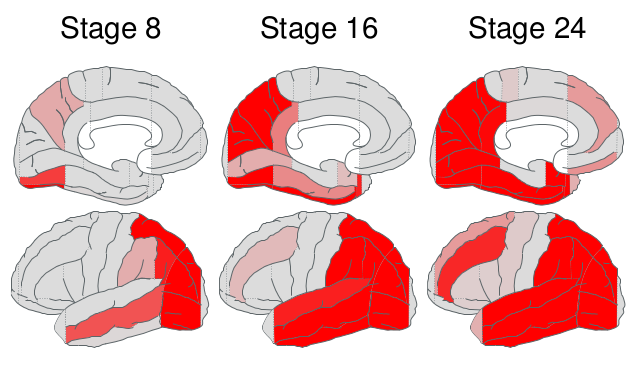
\includegraphics[height=\ovHeight]{ebm_thumb.png}
\end{subfigure}
}

\newcommand{\ovVWDPM}{
\begin{subfigure}{0.47\textwidth}
\centering
% \vspace{2.8em}
2. Developed Novel Spatio-temporal Model \\ (DIVE)\\
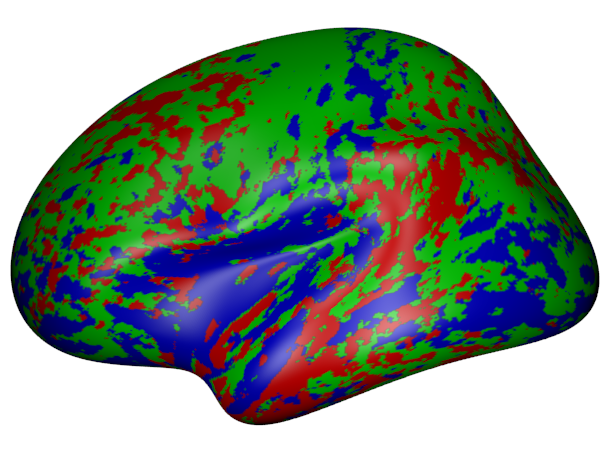
\includegraphics[height=\ovHeight]{\upgradeReportLoc/images/vwdpm/blend14_adniThavgFWHM0InithistCl3Pr0Ra1_VWDPMStd.png}
\end{subfigure}
}


\newcommand{\ovDKT}{
\begin{subfigure}{0.47\textwidth}
\centering
\vspace{2em}
3. Developed Novel Transfer Learning \\ method (DKT) \\
\vspace{0.5em}
\includegraphics[height=2.2cm]{\jointModellingDiseaseLoc/paper/figures/disease_knowledge_transfer.pdf}
\end{subfigure}
}


\newcommand{\ovTadpole}{
\begin{subfigure}{0.47\textwidth}
\centering
\vspace{-2em}
4. Organised TADPOLE Competition\\
\vspace{1em}
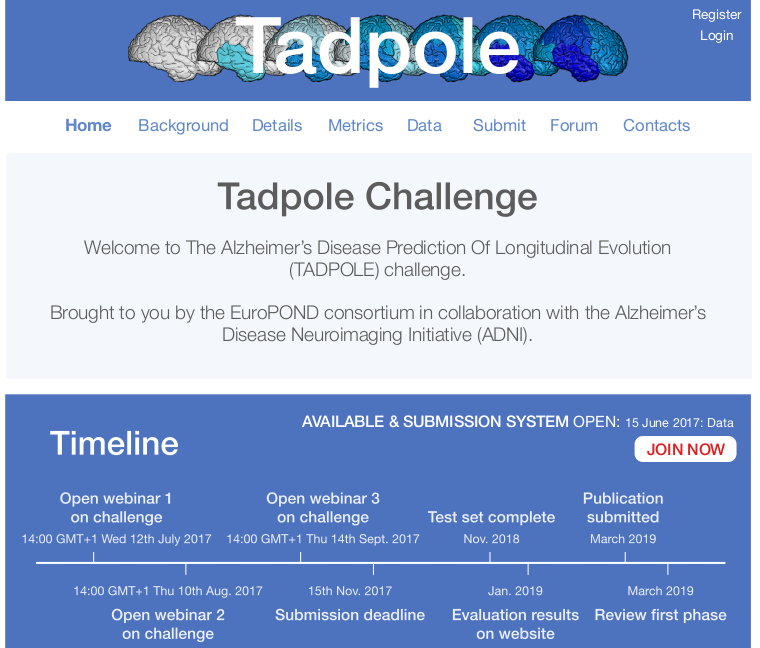
\includegraphics[height=1.2cm,valign=t]{\upgradeReportLoc/epsrcPres/tadpole} 
\end{subfigure}
}

\newcommand{\ovPainter}{
\begin{subfigure}{\textwidth}
\centering
\vspace{0.5em}
5. Created BrainPainter software\\
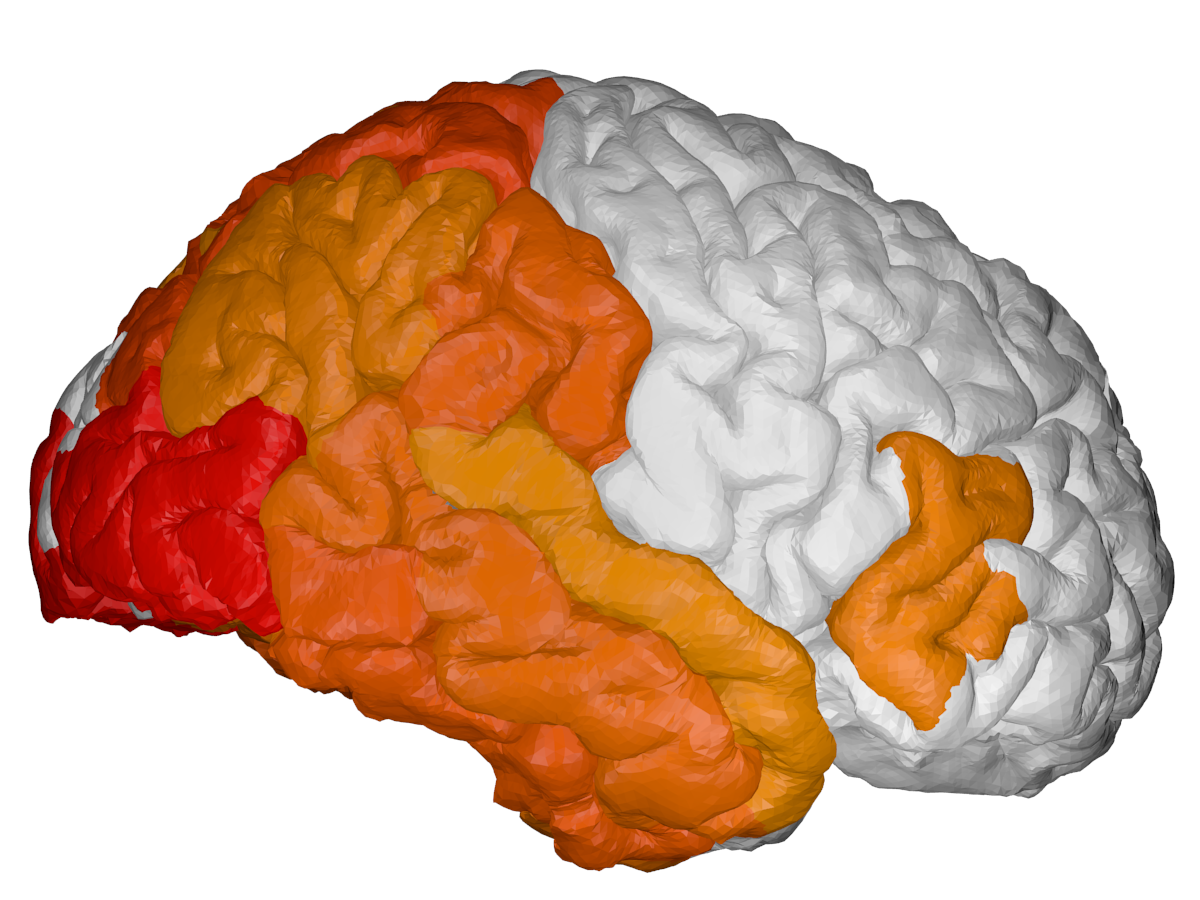
\includegraphics[height=1.5cm]{cortical-front_1}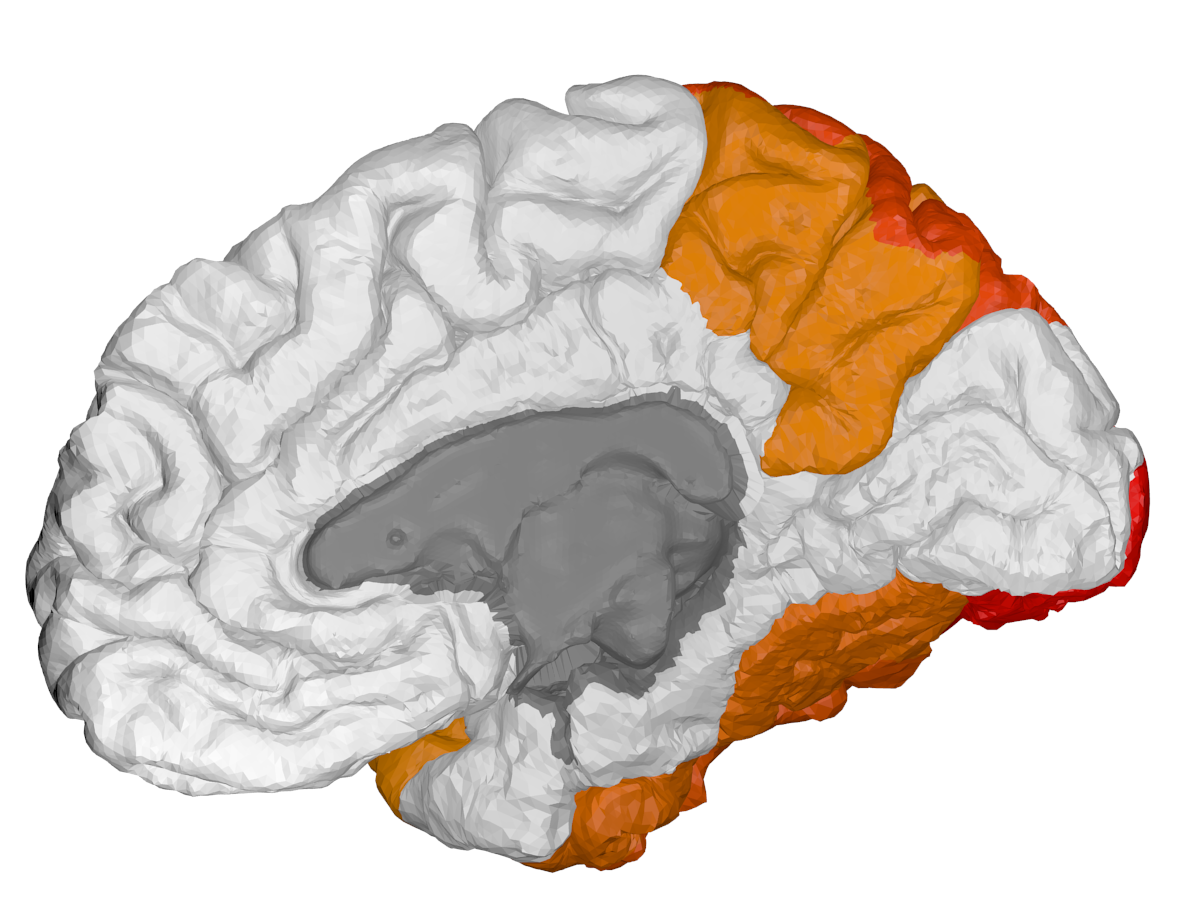
\includegraphics[height=1.5cm]{cortical-back_1}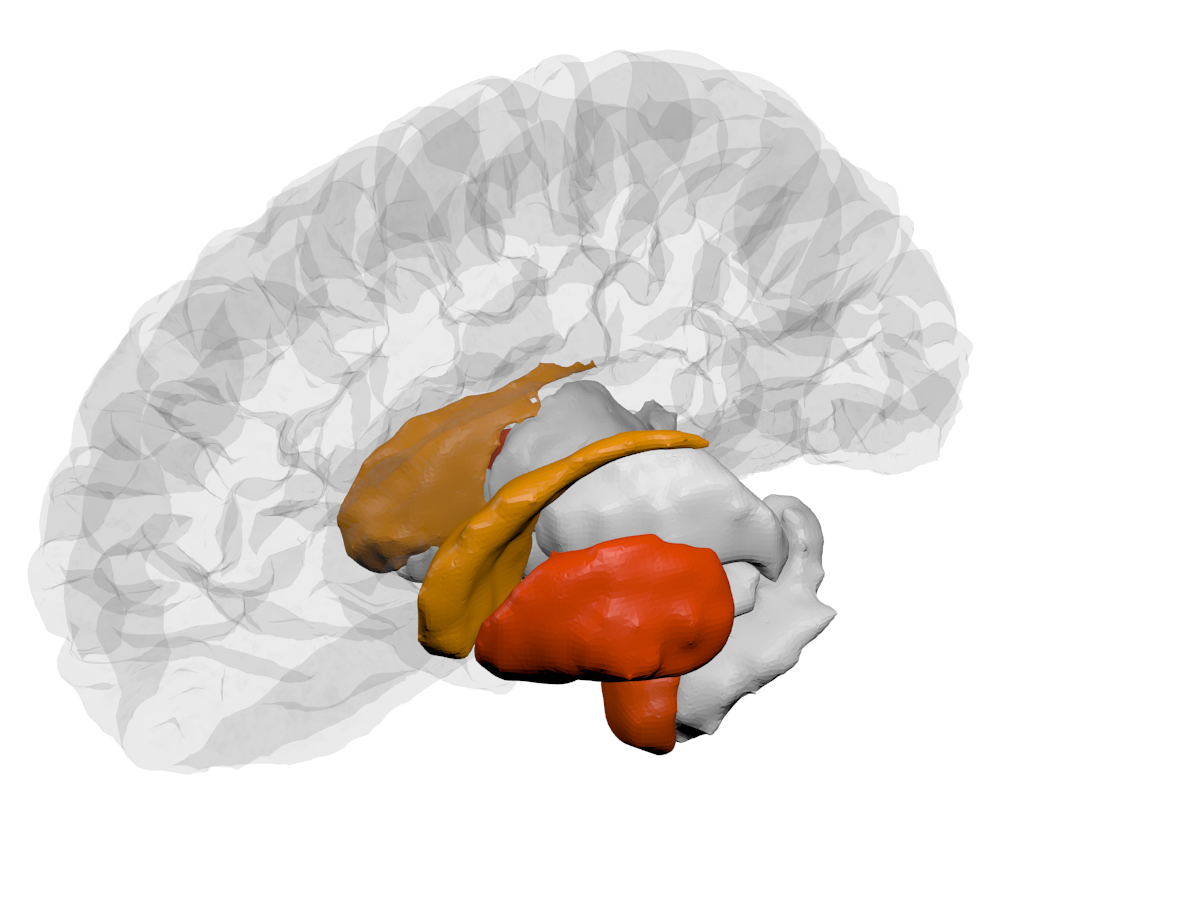
\includegraphics[height=1.5cm]{subcortical_1}
\end{subfigure}
}


\definecolor{light-gray}{gray}{0.6}


\newcommand{\inc}[1]{\includegraphics[width=\columnwidth, trim=4 4 4 4, clip]{#1}}
\newcommand{\incw}[2]{\includegraphics[width=#2\columnwidth, trim=4 4 4 4, clip]{#1}}
\newcommand{\inch}[2]{\includegraphics[height=#2, trim=4 4 4 4, clip]{#1}}

\begin{frame}{Machine Learning algorithms have achieved impressive milestones}

\begin{columns}[t]
\begin{column}{0.5\textwidth}
\centering
\begin{figure}
\vspace{-2em}

 Object detection (YOLO)
 \incw{yolo}{0.7}
 
 \vt
 
  Image Generation (StyleGAN2)
 \incw{stylegan_small}{0.7}
\end{figure}

\end{column}
\begin{column}{0.5\textwidth}
\centering
Text-to-Image Generation (DALL-E)
\inc{dalle2}
prompt: ``an armchair in the shape of an avocado''

\vspace{1.5em}

Text generation (GPT-3)
\inc{gpt3}
\end{column}

\end{columns}

\vo 

\begin{itemize}
 \item Largely driven by increases in data and compute
\end{itemize}
 
\end{frame}

\begin{frame}{Maching Learning holds great promise for improving healthcare}

\begin{columns}
 \begin{column}[t]{0.5\textwidth}
 \centering
 \textbf{\large{Diagnose with unprecedented accuracy}}
 \vo
  
  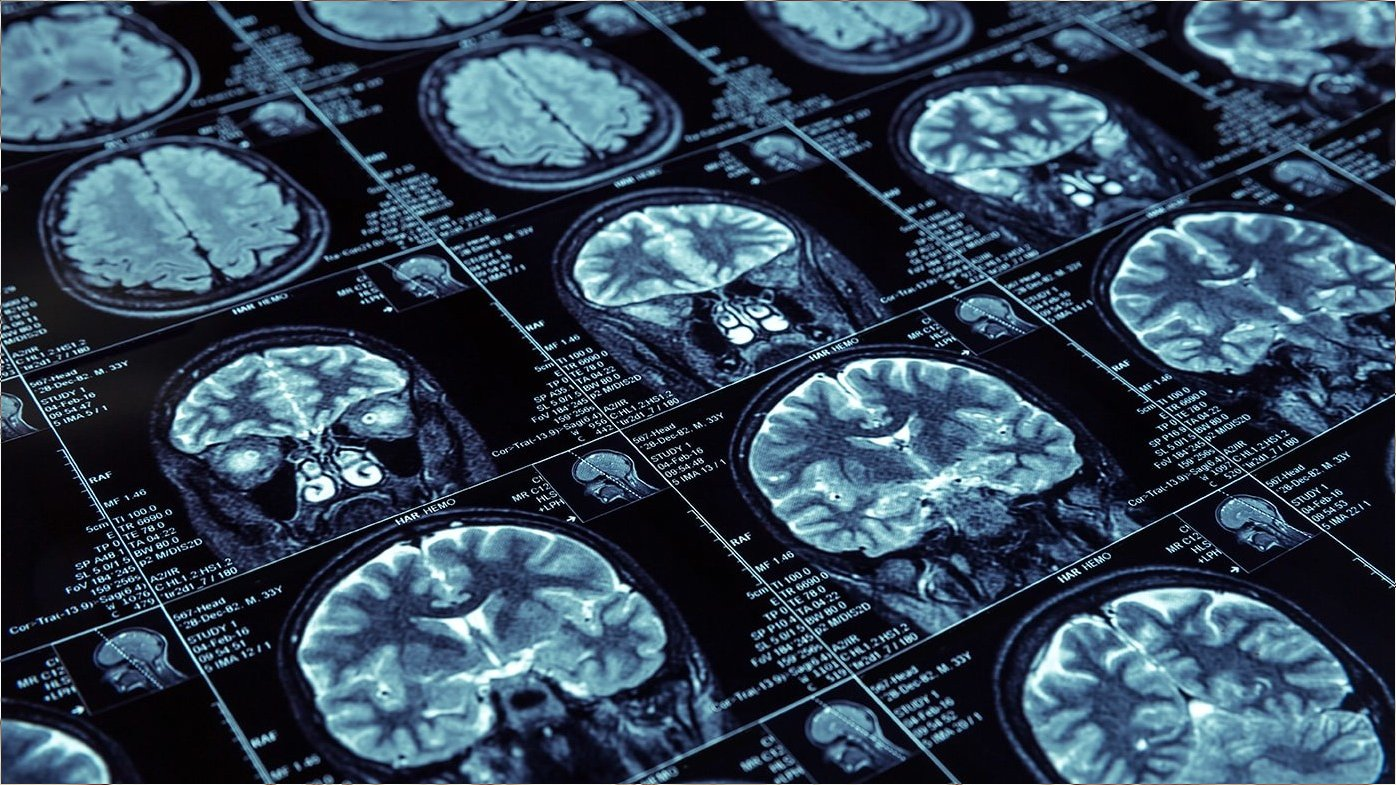
\includegraphics[width=0.75\columnwidth, trim=0 370 0 0, clip]{ai-diagnosis}
%  \incw{ml_predict_covid}{0.7} 
%  \inch{ai_radiology}{1.2cm}\inch{ai_radiology_pic}{1.2cm}

%  \incw{}
 
 \vt
 
%  \textbf{\large{Fast Diagnosis}}
 \inch{ai_12_ways}{1.3cm}\inch{ai_12_ways_pic}{1.3cm}
 
 
 \end{column}
 \begin{column}[t]{0.5\textwidth}
 \centering
 \textbf{\large{Augment doctors}}
 \vo
 
 \incw{ai_augment}{0.7}
 \vt
 
 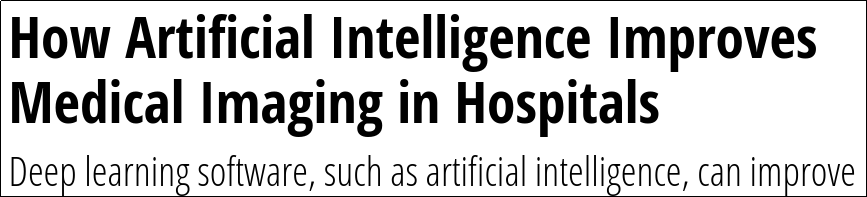
\includegraphics[height=0.9cm, trim=4 4 4 4, clip]{ai_improves_imaging_title2}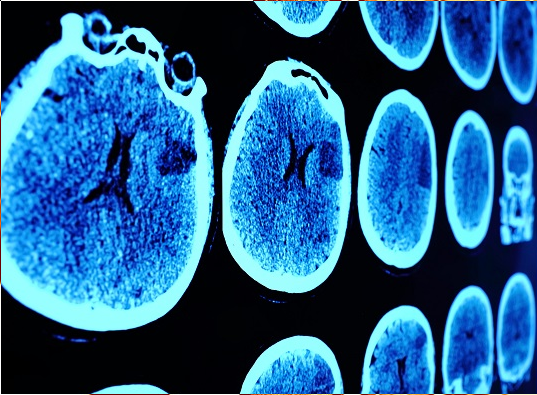
\includegraphics[height=0.9cm, trim=8 8 8 8, clip]{ai_improves_imaging_photo} 
 \vspace{2em}

  
 
 \end{column}

\end{columns}

\begin{center}
\textbf{\large{Improve patient healthcare and save lifes}}\\
\incw{ai_improves_care}{0.3} 
\end{center}


 
\end{frame}



\begin{frame}{However, such milestones have not been translated to medical applications}


\begin{columns}[t]
\begin{column}{0.5\textwidth}
\centering

\textbf{\large Prediction of clinical variables not always working} 

\vt

% \begin{itemize}
No algorithm/33 could predict cognitive scores in Alzheimer's (TADPOLE Challenge, Marinescu 2020)
% \end{itemize}
\vspace{2em}

\incw{tadpole_logo}{0.6}

\incw{tadpole_adas}{0.8}





% \end{itemize}


\end{column}
\begin{column}{0.5\textwidth}
\centering

% \begin{itemize}
\textbf{\large Generated images are crude, not high-resolution, mostly 2D}
% \end{itemize}

\vt

Brain MRI generation (Han, 2018)
\begin{figure}
\inc{brain-gen}

\vo

%Pneumonia segmentation (Wang, 2020)
%\incw{medseg}{0.7}

% Placenta segmentation (Wang, 2020)
% \incw{semi-automatic}{0.7}


\end{figure}
\end{column}
\end{columns}

 
 
\end{frame}


% Of 179 persons (average age, 86.9 years) with probable AD, 87.7% had pathologically confirmed AD, and 45.8% had mixed pathologies, most commonly AD with macroscopic infarcts (n = 54), followed by AD with neocortical LB disease (n = 19) and both (n = 8). 
% Of the 134 persons with MCI, 54.4% had pathologically diagnosed AD (58.7% amnestic; 49.2% nonamnestic); 19.4% had mixed pathologies (22.7% amnestic; 15.3% nonamnestic). Macroscopic infarcts without pathologically diagnosed AD accounted for 4.5% of probable AD, 13.3% of amnestic MCI, and 18.6% of nonamnestic MCI. Pure neocortical LB disease was uncommon in all persons with cognitive impairment (<6%). Microscopic infarcts (without macroscopic infarcts) were common as a mixed pathology, but rarely accounted for a clinical diagnosis of probable AD (n = 4) or MCI (n = 3).

\begin{frame}{Why are Machine Learning models not working on medical applications?}

\vspace{-1em}


\begin{columns}[t]
\begin{column}{0.5\textwidth}
\centering

\onslide<1-> \textbf{\large Lack of good labels}
% \begin{itemize}
% \item Lack of ground truth 

% ``Probable'' Alzheimer's disease diagnosis
\begin{itemize}
%  \item 

\onslide<1-> \item Alzheimer's diagnosis accuracy just 42\%

\onslide<1-> \begin{center}
\incw{ad_chart_schneider}{0.35}\\ 
\end{center}

\vspace{2.5em}

\onslide<2-> \item Labels are categorical instead of continuous\\
\vo
\onslide<2-> \incw{brain_prog_thresh}{1}

\end{itemize}

 \vspace{1em}
 

\end{column}
\begin{column}{0.5\textwidth}
\centering

\onslide<3-> \textbf{\large Lack of good input data/signal}
\begin{itemize}
\onslide<3-> \item Limited contrast

% \begin{itemize}
% \item Stroke scans with limited contrast
% \end{itemize}
\onslide<3-> \begin{center}
\incw{strokescan}{0.55}
\end{center}


\vspace{1em}

\onslide<4-> \item Low-resolution

\onslide<4-> \begin{center}
\incw{stroke_lowres2}{0.35} 
\end{center}



% \item Small datasets, inability to scale 
% 
% \begin{itemize}
% \item most have  $<100$ scans (Maier-Hein, 2018)
% \end{itemize}
% \incw{imgcount}{0.7}


\end{itemize}


\end{column}
\end{columns}

 
 
\end{frame}

\newcommand{\diagfld}{brgm_diagram}
\newcommand{\fstikz}[1]{\footnotesize{#1}}


\newcommand{\brgmprev}{
\begin{tikzpicture}[scale=0.5, every node/.style={scale=0.5}]

\def\rightimgX{4.5}

%top image center
\node (cxr_img) at (1, 3.5) {
\includegraphics[width=2cm]{\diagfld/brain_target}};
\node (cxr_text) at (1,4.75) {\footnotesize{Low Res.}};

%top image left
\node (blur_img) at (\rightimgX, 3.5) {\includegraphics[width=2cm]{\diagfld/brin_clean}};
\node (blur_text) at (\rightimgX,4.75) {\footnotesize{High Res.}};

%top image center
\node (cxr_img) at (1, 1) {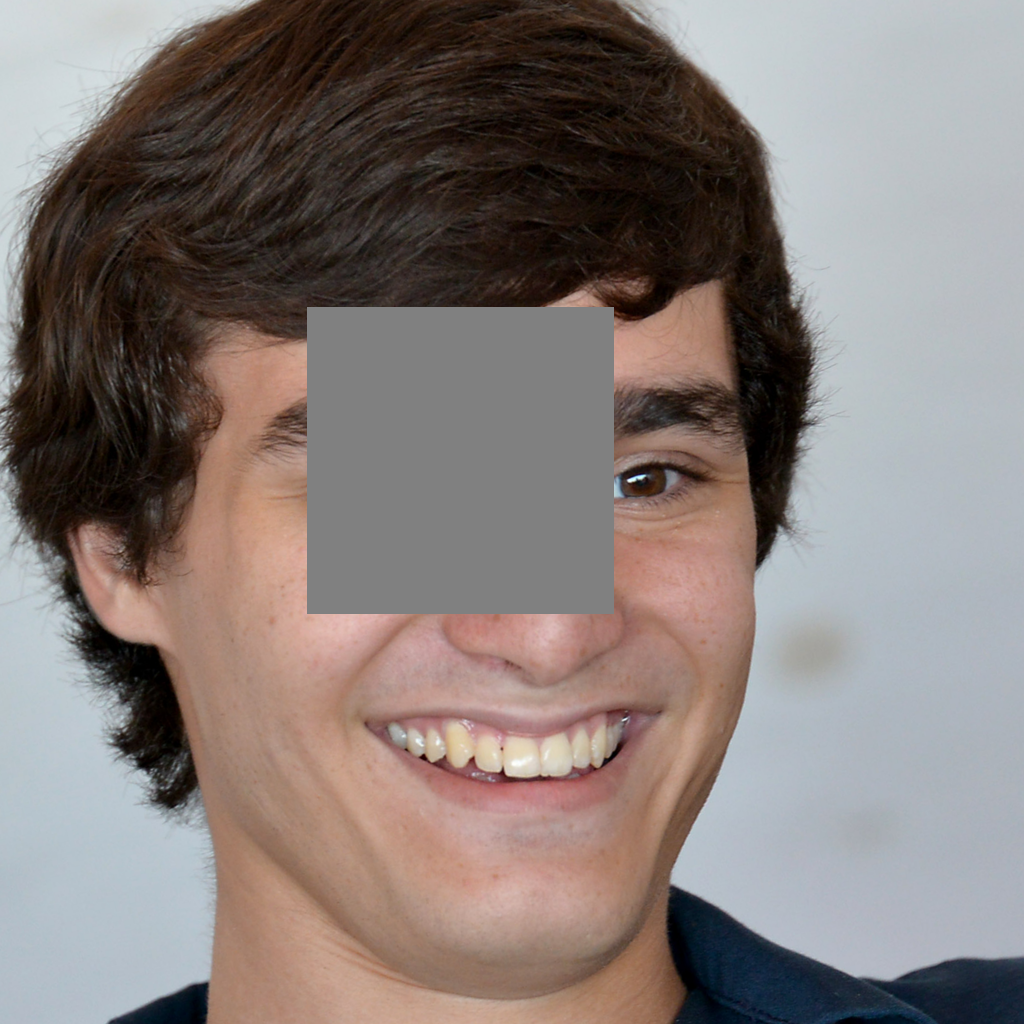
\includegraphics[width=2cm]{\diagfld/crop.png}};
%top image left
\node (blur_img) at (\rightimgX, 1) {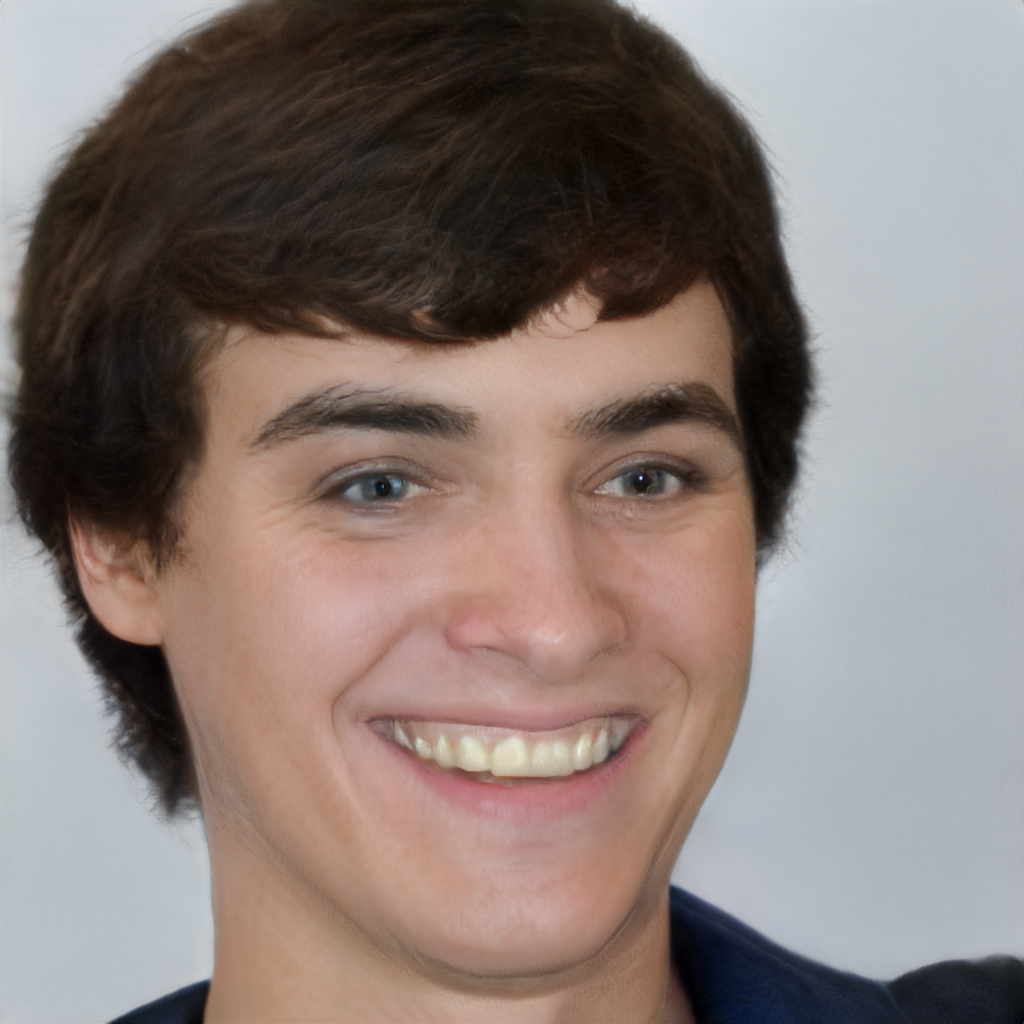
\includegraphics[width=2cm]{\diagfld/original.png}};

\node (left_img_top_out) at (2,3.5) {};
\node (right_img_top_in) at (\rightimgX - 1, 3.5) {};

\draw[->, thick]
(left_img_top_out)
to
(right_img_top_in) ;


\node (left_img_top_out_2) at (2,1) {};
\node (right_img_top_in_2) at (\rightimgX - 1, 1) {};

\draw[->, thick]
(left_img_top_out_2)
to
(right_img_top_in_2) ;


\node (left_img_top_in) at (2,2.5) {};
\node (right_img_top_out) at (\rightimgX - 1, 2.5) {};

\node (rng_text) at (2.75,3.75) {$f_1^{-1}(I)$};
\node (rng_text) at (2.75,3.25) {\fstikz{Learned}};
\node (rng_text) at (2.75,3) {\fstikz{Inverse}};
\node (rng_text) at (2.75,2.75) {\fstikz{Corruption}};

\node (rng_text) at (2.75,1.25) {$f_2^{-1}(I)$};

\end{tikzpicture}
}

\newcommand{\brgmours}{
\begin{tikzpicture}[scale=0.75, every node/.style={scale=0.75}]

\def\rightimgX{4.5}

%Top left
\filldraw[fill=gray!50!white, draw=black, label={Latent}] (-2,2.5) rectangle (-1.5,4.5);
\node (rng_text) at (-1.75,4.75) {\footnotesize{Latent}};
\node (rng_text) at (-1.75,3.5) {$w$};

%top image center
\node (cxr_img) at (1, 3.5) {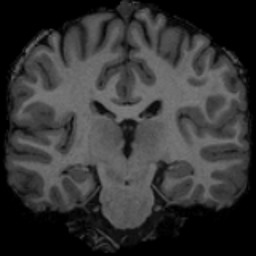
\includegraphics[width=2cm]{\diagfld/brain_clean}};
\node (cxr_text) at (1,4.75) {\footnotesize{High Res.}};

%top image right
\node (blur_img) at (\rightimgX, 3.5) {
\includegraphics[width=2cm]{\diagfld/brain_target}};
\node (blur_text) at (\rightimgX,4.75) {\footnotesize{Low Res.}};

\node (blur_img) at (\rightimgX+2.3, 3.5) {
\includegraphics[width=2cm]{\diagfld/brain_target}};
\node (blur_text) at (\rightimgX+2.3,4.75) {\footnotesize{Input}};

\draw[decoration={brace,mirror,raise=5pt},decorate]
  (4.5,2.5) -- node[below=6pt] {loss} (6.8,2.5);


\node (rng_top_out) at (-1.5,3.5) {};
\node (center_img_left_in) at (0, 3.5) {};

\draw[->, thick]
(rng_top_out)
to
(center_img_left_in) ;
@inproceedings{roth2005fields,
  title={Fields of experts: A framework for learning image priors},
  author={Roth, Stefan and Black, Michael J},
  booktitle={2005 IEEE Computer Society Conference on Computer Vision and Pattern Recognition (CVPR'05)},
  volume={2},
  pages={860--867},
  year={2005},
  organization={IEEE}
}
\node (left_img_top_out) at (2,3.5) {};
\node (right_img_top_in) at (\rightimgX - 1, 3.5) {};

\draw[->, thick]
(left_img_top_out)
to
(right_img_top_in) ;

\node (left_img_top_in) at (2,2.5) {};
\node (right_img_top_out) at (\rightimgX - 1, 2.5) {};

% \draw[->, dashed, blue, thick]
% (right_img_top_out)
% to [in=-60, out=-120]
% (left_img_top_in) ;


\node (left_img_bot_out) at (0,2.5) {};
\node (rng_bot_out) at (-1.5, 2.5) {};
\draw[->, dashed, red, thick]
(rng_bot_out)
to [in=-120, out=-60]
(left_img_bot_out);

\node (rng_text) at (-0.75,3.75) {$G(w)$};
\node (rng_text) at (-0.75,3.25) {\fstikz{Image}};
\node (rng_text) at (-0.75,3) {\fstikz{Generation}};

\node (rng_text) at (2.75,3.75) {$f_1$};
\node (rng_text) at (2.75,3.25) {\fstikz{Known}};
\node (rng_text) at (2.75,3) {\fstikz{Corruption}};

\node (rng_text) at (-0.75,1.75) {\fstikz{Learned a-priori}};
\node (rng_text) at (-0.75,1.5) {\fstikz{given High Res Data}};
% \node (rng_text) at (-0.75,1.25) {\fstikz{given High Res Data}};

\node (rng_text) at (-0.5,0.75) {\fstikz{Can be redone}};
\node (rng_text) at (-0.5,0.5) {\fstikz{using the same $G(w)$}};
\node (rng_text) at (-0.5,0.25) {\fstikz{for multiple $f_i$}};


% \node (rng_text) at (2.75,1.75) {\fstikz{Optimized at}};
% \node (rng_text) at (2.75,1.5) {\fstikz{Test Time}};



\node (left_img_center_out) at (1,2.5) {};
\node (right_bot_out_extra) at (3.9 - 1, 1) {};
\draw[->, thick]
(left_img_center_out)
to [in=90, out=-90]
(1,1) 
to [out=0, in=180]
(right_bot_out_extra);

\node (right_bot_out_extra_2) at (3.9 - 1, 0.5) {};
\draw[->, thick]
(left_img_center_out)
to [in=90, out=-90]
(1,0.5) 
to [out=0, in=180]
(right_bot_out_extra_2);


\node (rng_text) at (1.75,1.25) {$f_2$};
\node (rng_text) at (1.75,0.75) {$f_3$};
\node (rng_text) at (1.75,0.25) {$\vdots$};


\node (blur_img) at (3.5+0.5, 0.5) {
\includegraphics[width=1cm]{\diagfld/brain_kspace.png}};
\node (blur_img) at (3.5, 1.0) {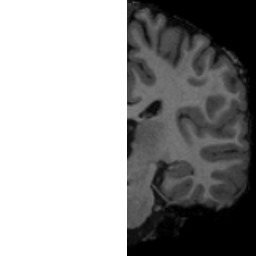
\includegraphics[width=1cm,frame]{\diagfld/brain_inpaint}};

\end{tikzpicture}
}


\newcommand{\brgmoursshort}{
\begin{tikzpicture}[scale=0.75, every node/.style={scale=0.75}]

\def\rightimgX{4.5}

%Top left
\filldraw[fill=gray!50!white, draw=black, label={Latent}] (-2,2.5) rectangle (-1.5,4.5);
\node (rng_text) at (-1.75,4.75) {\footnotesize{Latent}};
\node (rng_text) at (-1.75,3.5) {$w$};

%top image center
\node (cxr_img) at (1, 3.5) {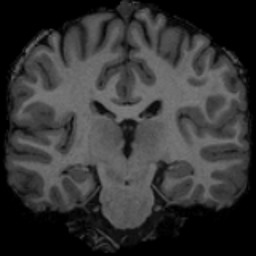
\includegraphics[width=2cm]{\diagfld/brain_clean}};
\node (cxr_text) at (1,4.75) {\footnotesize{High Res.}};

%top image right
\node (blur_img) at (\rightimgX, 3.5) {
\includegraphics[width=2cm]{\diagfld/brain_target}};
\node (blur_text) at (\rightimgX,4.75) {\footnotesize{Low Res.}};

\node (rng_top_out) at (-1.5,3.5) {};
\node (center_img_left_in) at (0, 3.5) {};

\draw[->, thick]
(rng_top_out)
to
(center_img_left_in) ;

\node (left_img_top_out) at (2,3.5) {};
\node (right_img_top_in) at (\rightimgX - 1, 3.5) {};

\draw[->, thick]
(left_img_top_out)
to
(right_img_top_in) ;

\node (left_img_top_in) at (2,2.5) {};
\node (right_img_top_out) at (\rightimgX - 1, 2.5) {};

\node (left_img_bot_out) at (0,2.5) {};
\node (rng_bot_out) at (-1.5, 2.5) {};


% \node (rng_text) at (-0.75,3.75) {$G(w)$};
\node (rng_text) at (-0.75,3.25) {\fstikz{Image}};
\node (rng_text) at (-0.75,3) {\fstikz{Generation}};

% \node (rng_text) at (2.75,3.75) {$f_1$};
\node (rng_text) at (2.75,3.25) {\fstikz{Known}};
\node (rng_text) at (2.75,3) {\fstikz{Corruption}};

\end{tikzpicture}
}





\begin{frame}{What can we do?}


\vspace{-8em}
\begin{columns}[t]
\begin{column}{0.5\textwidth}
\centering

\textbf{\large Lack of good labels}

% \begin{itemize}
% \item Alzheimer's diagnosis accuracy just 42\%
% % \begin{itemize}
% %  \item Infer continuous disease staging
% %  
% % %  \incw{severity}{0.7}
% % \end{itemize}
% 
%  \vspace{2em}
%  
%  \item Noisy labels
% % \begin{itemize}
% %    \item Infer true labels from noisy ones  
% % \end{itemize}
% 
% % \incw{goldstandard}{0.7}
% \end{itemize}

\vspace{2em}

% \vspace{-4em}

\end{column}
\begin{column}{0.5\textwidth}
\centering

\textbf{\large Lack of good input data/signal}

% \vspace{-1.5em}

% \begin{itemize}
% \item Lack of good input data
% 
% % \begin{itemize}
% %   \item Reconstruct better images
% % \end{itemize}
% % \incw{strokescan}{0.7}
% 
% \vspace{0.5em}
% 
% \item Small datasets, inability to scale 
% % \begin{itemize}
% % \item Acquire more data
% % \item Design algorithms for small datasets
% % % \begin{itemize}
% % %  \item Transfer learning
% % %  \item Few-shot or Zero-shot learning
% % % \end{itemize}
% % 
% % \end{itemize}
% % \incw{imgcount}{0.7}
% \end{itemize}

\vspace{2em}




\end{column}
\end{columns}


\begin{columns}[t]
\begin{column}{0.5\textwidth}
\centering

Solution: Unsupervised Learning of Continuous Dynamics\\
= Disease Progression Modelling\\
\vo

%Time-series model with\\ latent disease stage\\
% = Disease Progression Model\\
%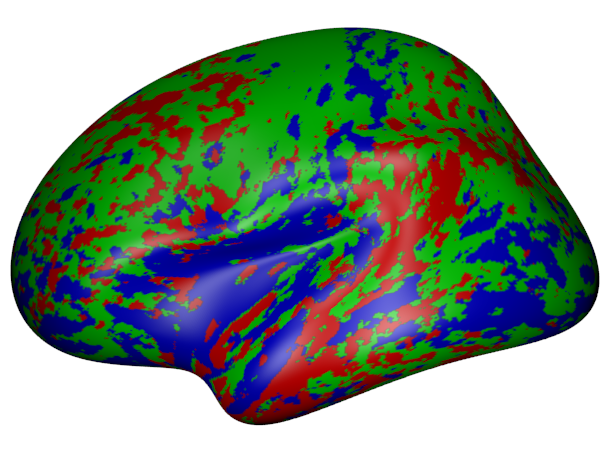
\includegraphics[height=\ovHeight]{\upgradeReportLoc/images/vwdpm/blend14_adniThavgFWHM0InithistCl3Pr0Ra1_VWDPMStd.png}
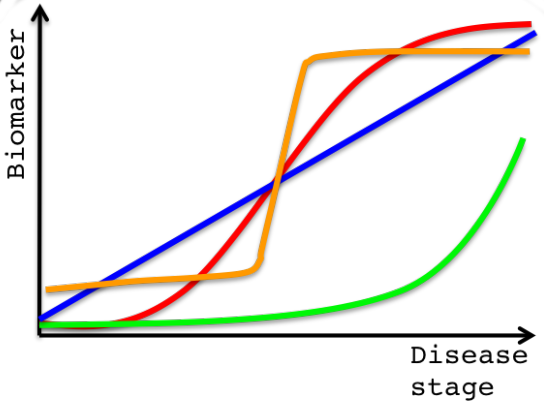
\includegraphics[height=3cm]{dpm_small}

\end{column}
\begin{column}{0.5\textwidth}
\centering

Solution: Image Reconstruction\\ using Deep Generative Models\\
\vo
% 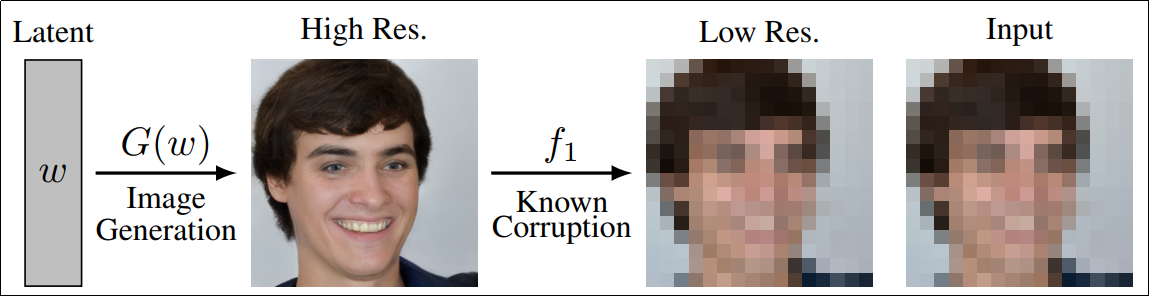
\includegraphics[height=2cm, trim=6 6 6 6,clip]{brgm_diagram_small}
\brgmoursshort

\end{column}
\end{columns}

\end{frame}


\begin{frame}{Outline}




\begin{enumerate}
 \item Disease progression modelling of Alzheimer's disease 
 \begin{enumerate} 
  \item Towards unsupervised clustering of biomarker trajectories\\
 \end{enumerate}
   
% 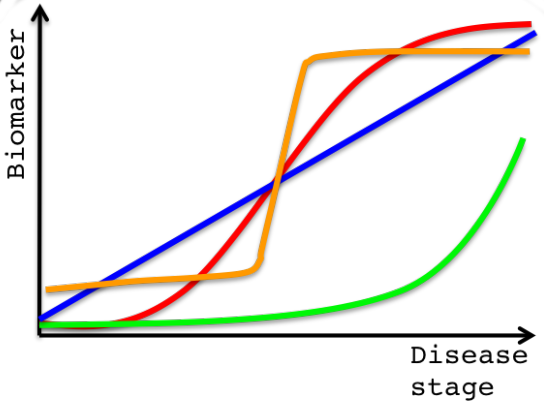
\includegraphics[height=2cm]{dpm_small} 
% \vt 
%  \item Unsupervised clustering of trajectories
 
   \begin{tikzpicture}[scale=1]
     \node (roi) at (0,0) {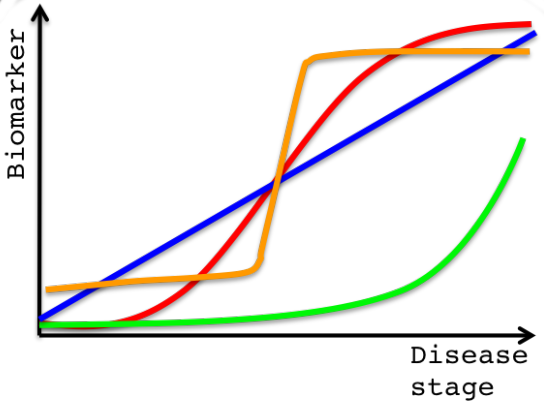
\includegraphics[height=1.5cm]{dpm_small}};
     \node (vw) at (4,0) {\includegraphics[height=1.5cm]{\voxFld/selected_resfiles/adniPet/atrophyExtent24_adniPetInitk-meansCl18Pr1Ra1_VDPM_MRF.png}};
     \draw[line width=1.5,->] (roi) -> (vw);
  \end{tikzpicture}
  
  \vt

 \item Image Reconstruction using Deep Generative Models\\
%  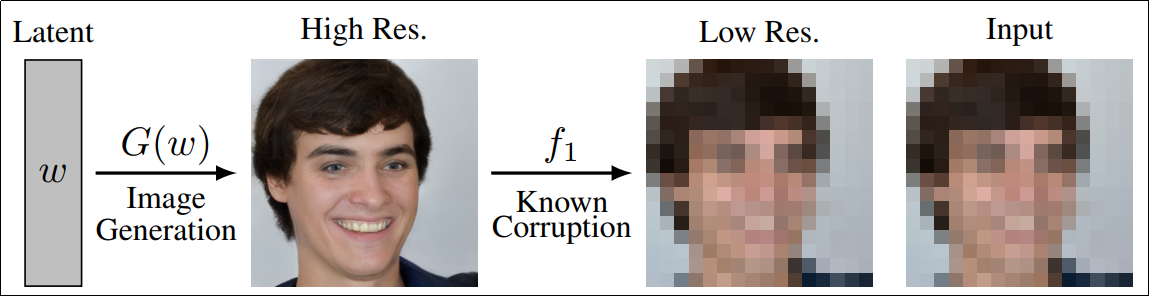
\includegraphics[height=1.5cm, trim=6 6 300 6,clip]{brgm_diagram_small}
\brgmoursshort
\vt
 
  \item Future work\\

\end{enumerate}
 


\end{frame}


\begin{frame}{Outline}

\begin{enumerate}
 \item \textbf{Disease progression modelling of Alzheimer's disease}
 \begin{enumerate} 
  \item Towards unsupervised clustering of biomarker trajectories\\
 \end{enumerate}
   
% 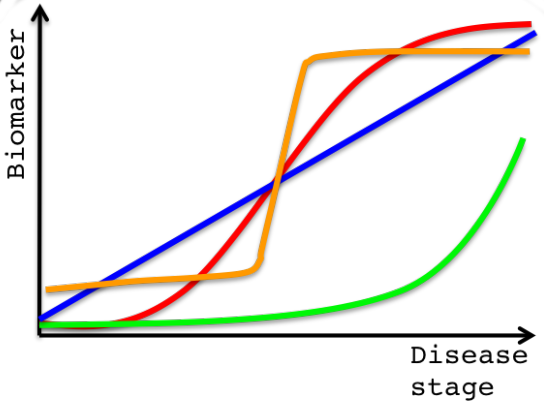
\includegraphics[height=2cm]{dpm_small} 
% \vt 
%  \item Unsupervised clustering of trajectories
 
   \begin{tikzpicture}[scale=1]
     \node (roi) at (0,0) {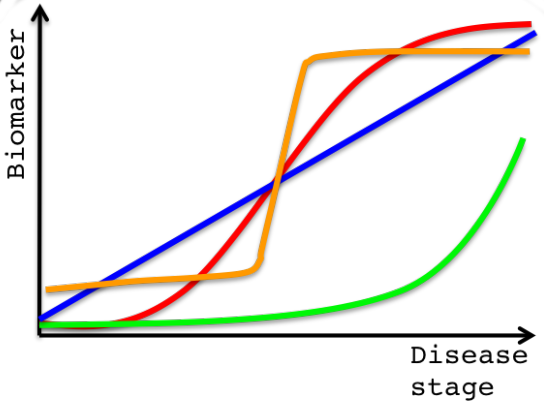
\includegraphics[height=1.5cm]{dpm_small}};
     \node (vw) at (4,0) {\includegraphics[height=1.5cm]{\voxFld/selected_resfiles/adniPet/atrophyExtent24_adniPetInitk-meansCl18Pr1Ra1_VDPM_MRF.png}};
     \draw[line width=1.5,->] (roi) -> (vw);
  \end{tikzpicture}
  
  \vt

 \item Image Reconstruction using Deep Generative Models\\
%  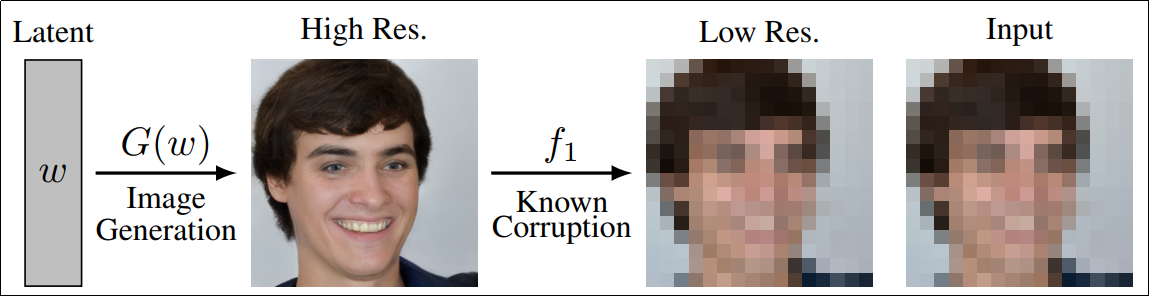
\includegraphics[height=1.5cm, trim=6 6 300 6,clip]{brgm_diagram_small}
\brgmoursshort
\vt
 
  \item Future work\\

\end{enumerate}
\end{frame}


% 
% \begin{frame}
% \frametitle{Aim: Estimate the progression of Alzheimer's disease}
% 
% Estimate the progression of Alzheimer's disease 
% 
% 
% 
% \end{frame}


\begin{frame}
\frametitle{Alzheimer's Disease is a Devastating Disease}

\vspace{-1em}
\begin{itemize}
 \item 46 million people affected worldwide
 
  \begin{figure}
 \centering
%   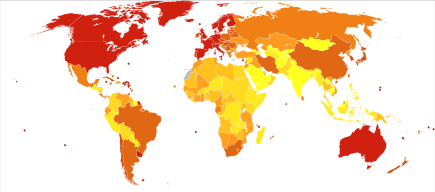
\includegraphics[height=3cm]{adPrelavence}
  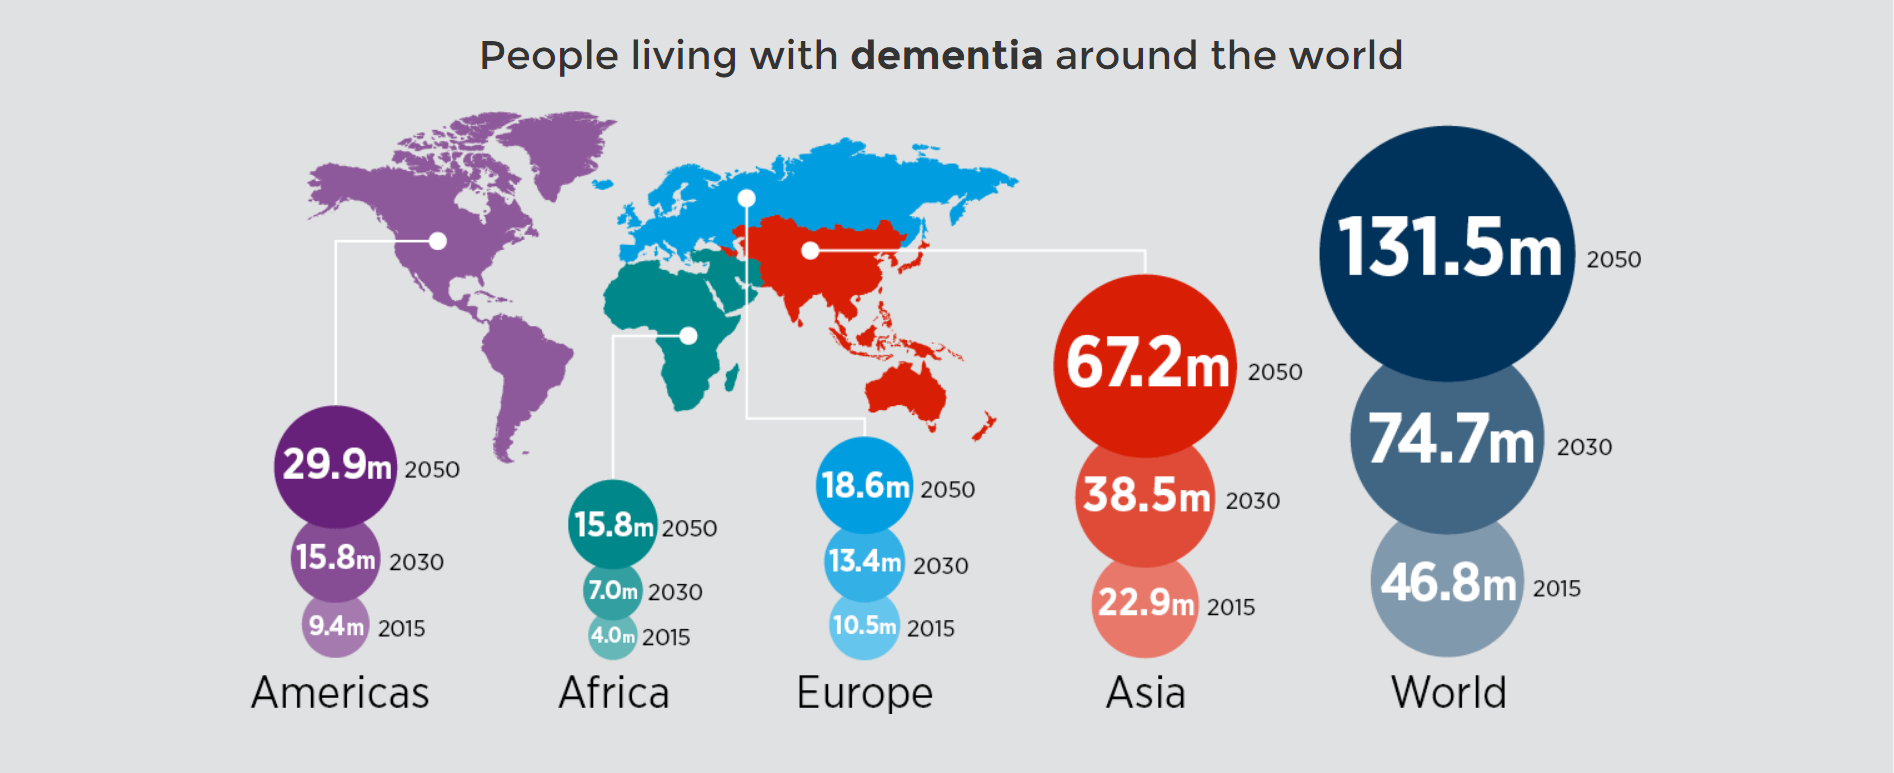
\includegraphics[height=4cm]{adPrevalanceIncreasing}
 \end{figure}
 
 \onslide<2-> \item No treatments available that stop or slow down cognitive decline
 \onslide<2-> \item Q: Why did clinical trials fail? A: Treatments were not administered early enough 
 \vspace{1em}
 \onslide<3-> \item Q: How can we then identify subjects \textbf{early} in order to administer treatments? 
 \onslide<3-> \item A: Biomarkers ...
 

\end{itemize}

\vspace{-1em}

\end{frame}

% Also say that we cannot build the model on age
\begin{frame}
\frametitle{Biomarker Evolution creates a Unique Disease Signature\\
that can be used for Staging Individuals in Clinical Trials}
% explain what are the challenges

\begin{figure}
\centering 
\vspace{1em}
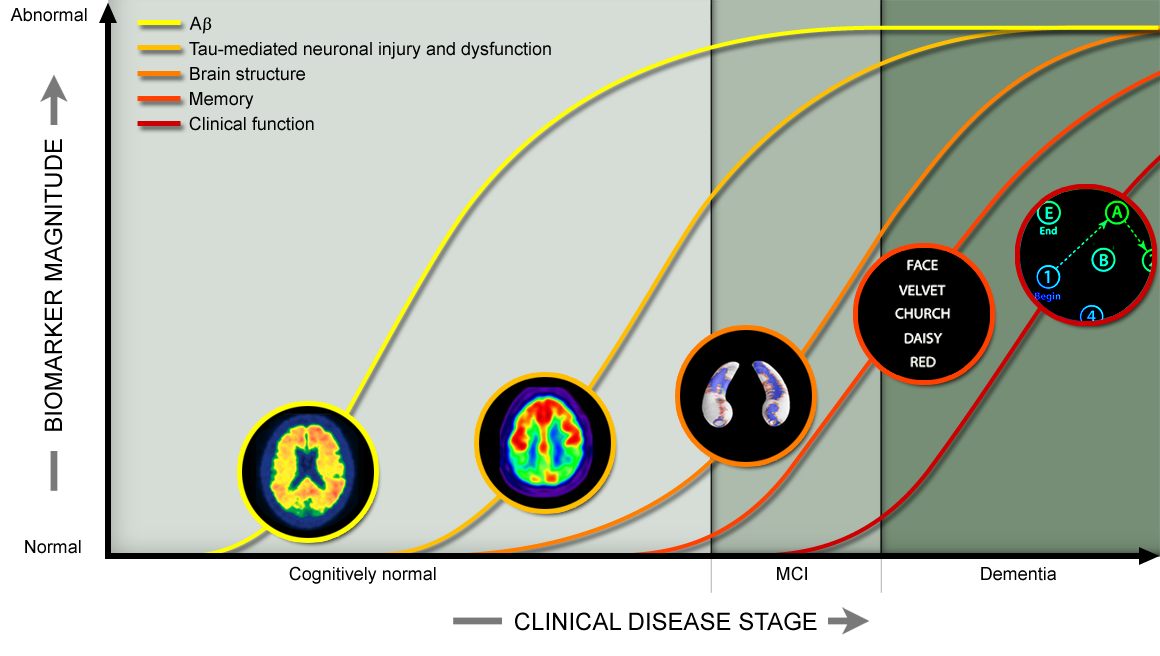
\includegraphics[height=5cm]{adniDiseaseProgression}
\hspace{-4em}ADNI website 

\end{figure}


\begin{itemize}
 \item Problem: the X-axis is inferred, we don't observe it directly
 \item Accurate disease staging $\rightarrow$ better patient stratification
 \item Problem: This is a "hypothetical" (i.e. qualitative) disease progression model
 \item Why construct a quantitative model? 
\end{itemize}

\end{frame}


% \section{Disease Progression Modelling}



\begin{frame}
\frametitle{Benefits of Quantitative Disease Progression Models}

\begin{overprint}
 \onslide<1>\begin{figure}
 \centering
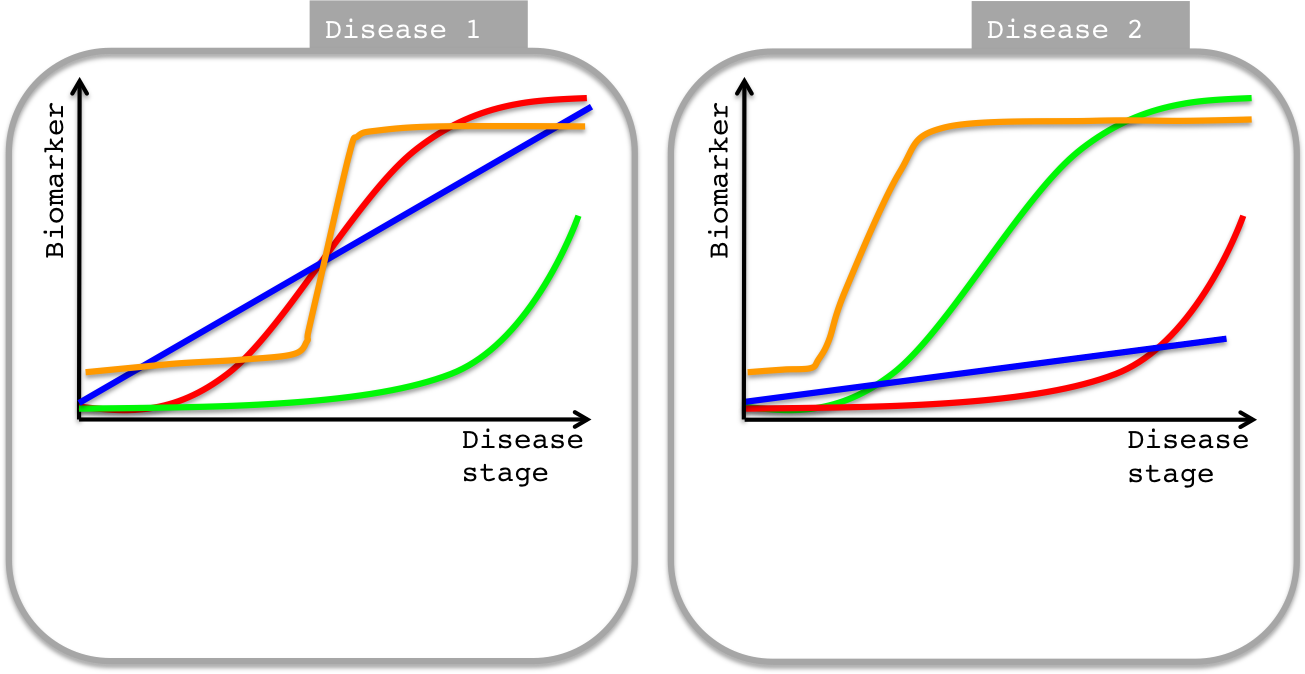
\includegraphics[height=5cm,trim=0 0 650 0,clip]{dpmDiffDiag1.png}
\end{figure}

\onslide<2> \begin{figure}
 \centering
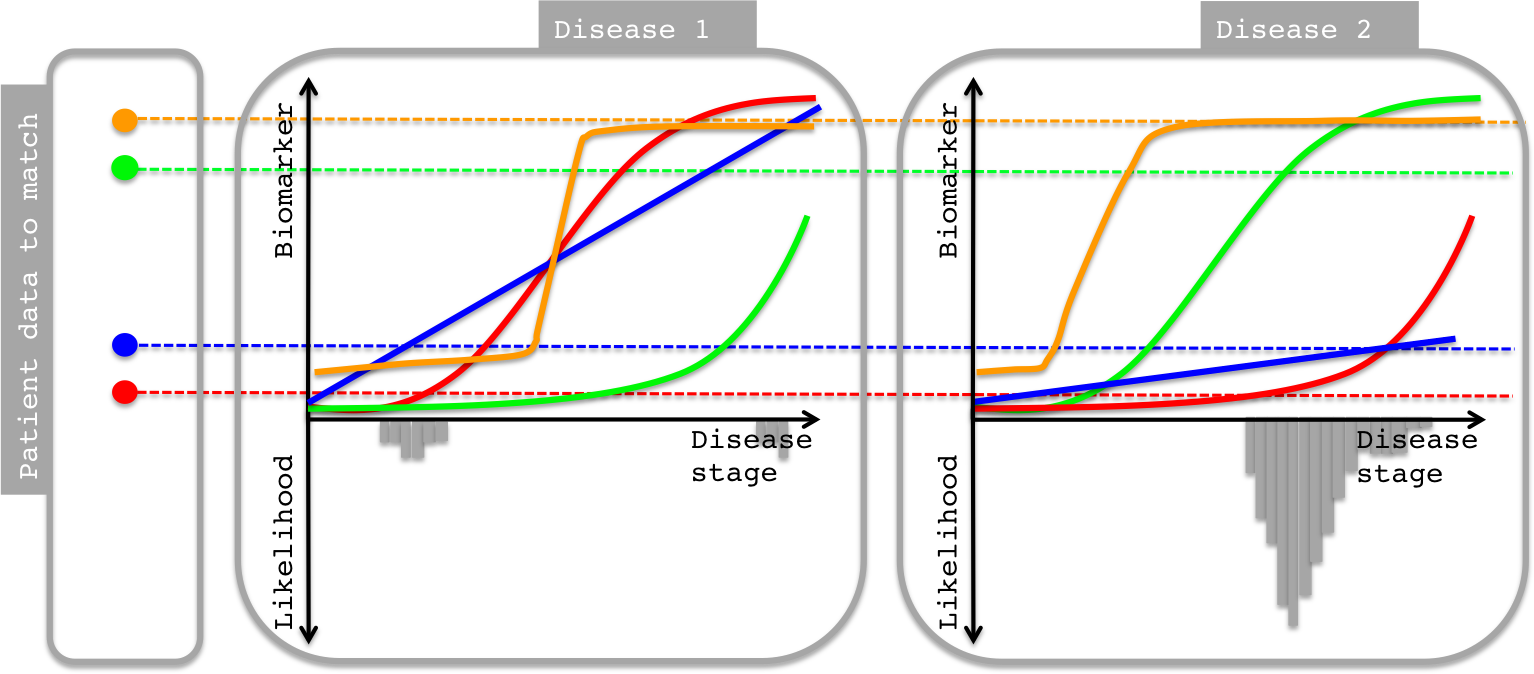
\includegraphics[height=5cm,trim=0 0 650 0,clip]{dpmDiffDiag2.png}
\end{figure}

\onslide<3-> \begin{figure}
 \centering
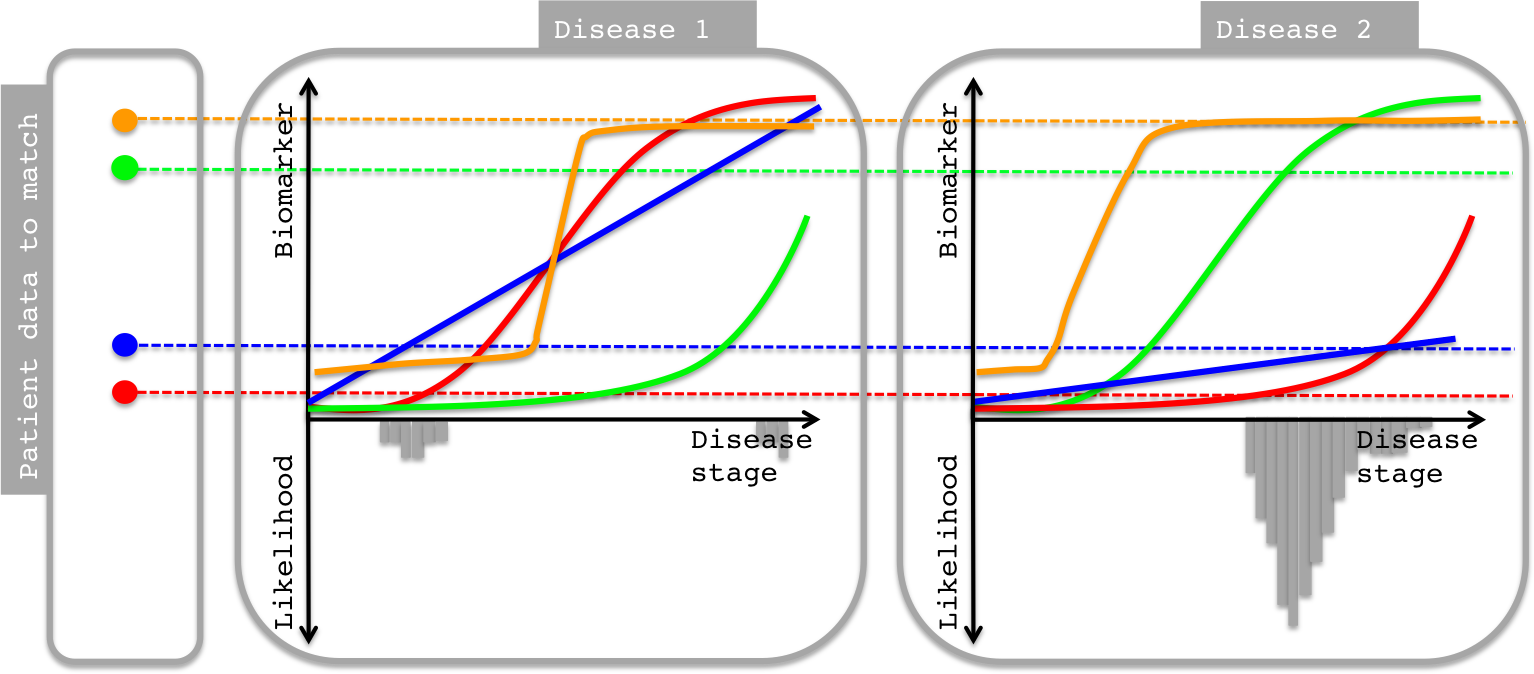
\includegraphics[height=5cm,trim=0 0 0 0,clip]{dpmDiffDiag2.png}
\end{figure}

\end{overprint}

\vspace{1em}
\begin{itemize}
 \onslide<1-> \item Basic biological insight
 \onslide<2-> \item Staging can help stratification in clinical trials
 \onslide<3-> \item Differential diagnosis and prognosis
 
 \vspace{1.5em}
%  \onslide<4-> \item[] How can we build such a disease progression model?
\end{itemize}

\end{frame}





% \begin{frame}[label=current]
% \frametitle{My PhD Contributions}
% 
% \begin{figure}
% \centering
% 
% 
% \ovEBM
% \ovVWDPM
% 
% \ovDKT
% \ovTadpole
% 
% \ovPainter
% 
% \end{figure}
% 
% \end{frame}




% \section{DIVE}
% 
% \begin{frame}
% \frametitle{My PhD Contributions}
% 
% %% new slide
% 
% \begin{figure}
% \centering
% 
% 
% {\transparent{0.4} 
% \ovEBM 
% }
% \ovVWDPM
% 
% {\transparent{0.4} 
% \ovDKT
% \ovTadpole
% 
% \ovPainter
% }
% 
% \end{figure}
% 
% \end{frame}


\begin{frame}
\frametitle{Aim: Build a Disease Progression Model of Pathology over the Brain that Avoids Limitations of Previous Models}


\newcommand{\aimImgScale}{0.8}
\newcommand{\mnpHeight}{3cm}

\vspace{-2em}

% FWHM0 avg thickness map MCI & AD
\begin{figure}[h]
  \centering
  \begin{minipage}[t][\mnpHeight][t]{0.3\textwidth}
   \centering
   Avoids pre-defined ROI parcellation\\
  \begin{tikzpicture}[scale=1]
    \node[inner sep=0] (image) at (0,0) {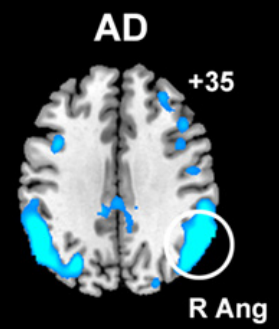
\includegraphics[width=0.5\textwidth,trim=0 0 26 0,clip]{seeley_2009_topleft.png}}; 
  \end{tikzpicture}
%     \caption{}
%       \label{fig:adniClust}
  \end{minipage}
   \begin{minipage}[t][\mnpHeight][t]{0.3\textwidth}
  \centering
  Avoids simplistic spatial correlation structure\\
%   \vspace{1em}
  \begin{tikzpicture}[scale=1]
    \node[inner sep=0] (corr_text) at (0,0) {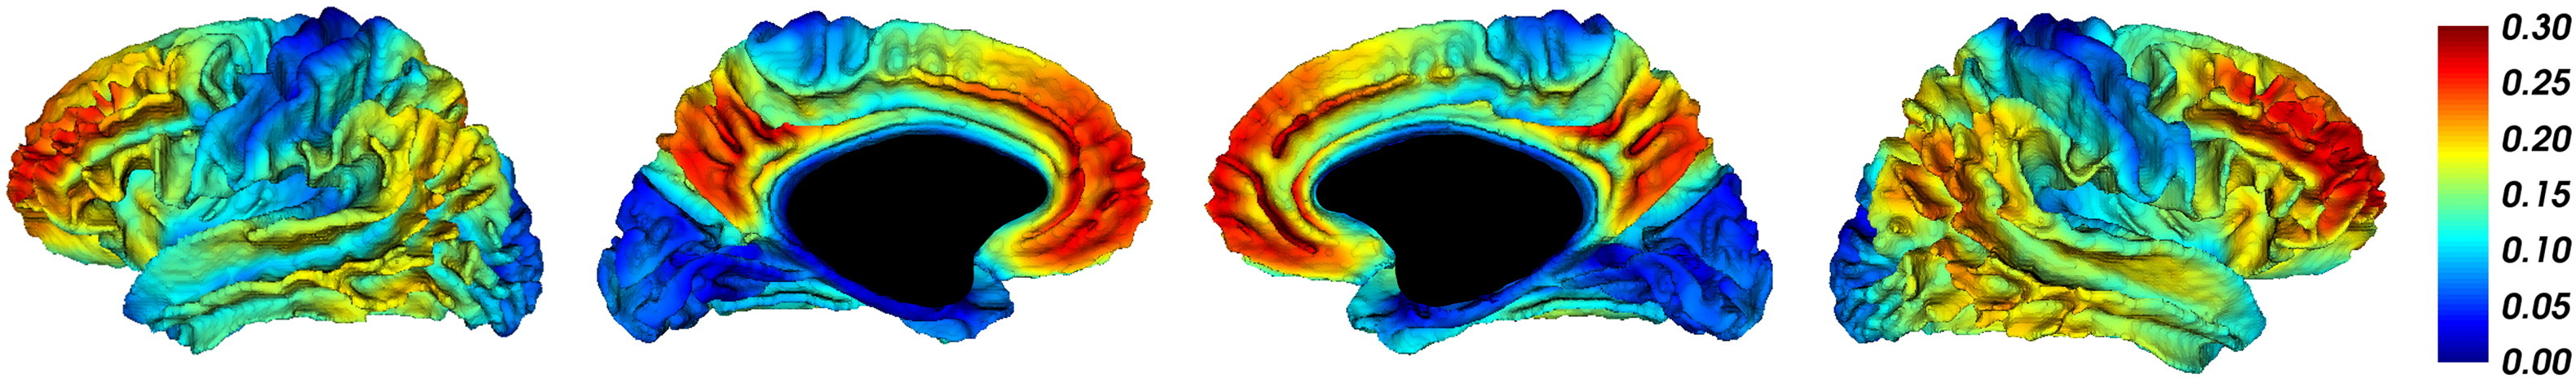
\includegraphics[width=\aimImgScale\textwidth, trim=0 0 360 0, clip]{bilgel_neuroimage}};
  \end{tikzpicture}
  \vspace{0.5em}
  \end{minipage}
   \begin{minipage}[t][\mnpHeight][t]{0.3\textwidth}
  \centering
  Avoids simplistic biomarker trajectories
  \begin{tikzpicture}[scale=1]
    \node[inner sep=0] (corr_text) at (0,0) {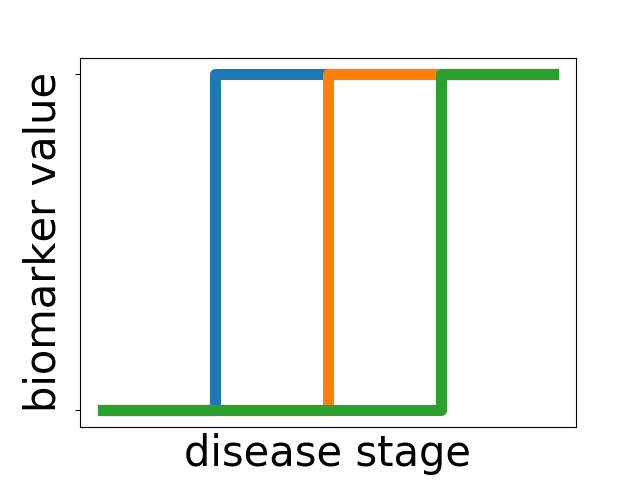
\includegraphics[width=\aimImgScale\textwidth,trim=0 0 0 30,clip]{biomkStepFunctions}};
  \end{tikzpicture}
  \end{minipage}
\end{figure}

\vfill

This leads to a technique that simultaneously:
\begin{itemize}
 \item parcellates the brain into disconnected components that undergo similar progression
 \item estimates biomarker trajectories
\end{itemize}


\end{frame}


\begin{frame}
\frametitle{Motivation: Correlate with brain networks + better prediction/staging}


\begin{itemize}
 \item \textbf{Aim}: Move from ROI-based analysis to voxelwise/vertexwise
\end{itemize}

\begin{figure}
 \centering
  \begin{tikzpicture}[scale=1]
     \node (roi) at (0,0) {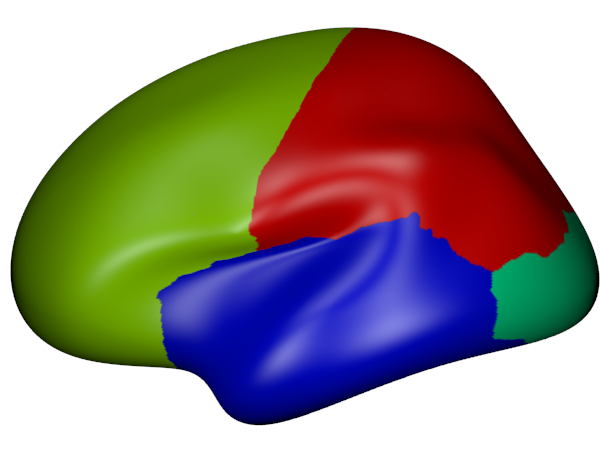
\includegraphics[scale=0.10]{clust24_drcThFWHM0InitfsurfCl4Pr0Ra1Mrf5_VWDPMStaticPCA.png}};
     \node (vw) at (4,0) {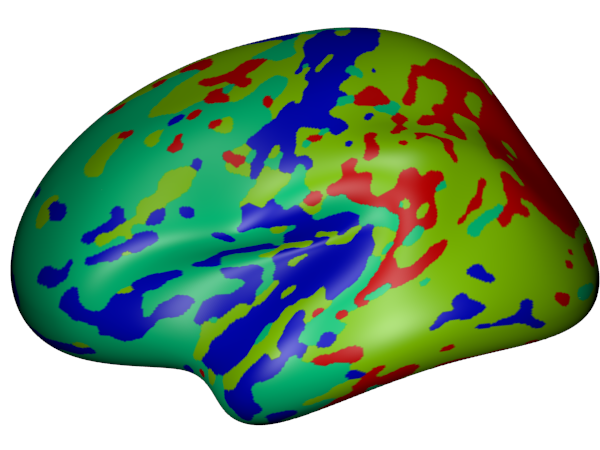
\includegraphics[scale=0.10]{clust24_drcThFWHM0Initk-meansCl4Pr0Ra1Mrf5_VDPM_MRFPCA.png}};
     \draw[line width=1.5,->] (roi) -> (vw);
  \end{tikzpicture}
\end{figure}



\begin{figure}
\begin{subfigure}{0.48\textwidth}
%\textbf{Motivation}:
\begin{enumerate}
\item Atrophy correlates with functional networks, which are not spatially connected (Seeley et al., Neuron, 2009)
\vspace{2em}
\item Better biomarker prediction and disease staging
\end{enumerate}
\end{subfigure}
% \hspace{1em}
\begin{subfigure}{0.5\textwidth}
\centering 
% \vspace{-5em}
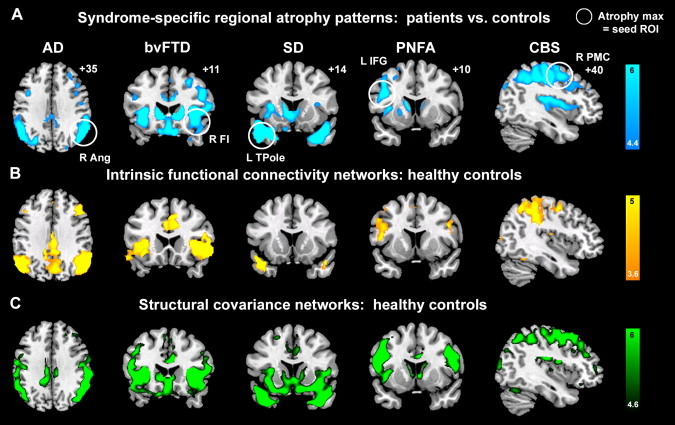
\includegraphics[width=\textwidth, right, trim=0 85 0 0, clip]{seeley_connectivity_overlap.jpg}
\caption{Seeley et al., Neuron, 2009}
\end{subfigure}

\end{figure}

\vfill

\vspace{-3em}


\end{frame}





\begin{frame}
\frametitle{Background - Disease Progression Modelling}

\newcommand{\mnpHeight}{3cm}

\vspace{-3em}
% \textbf{Background}:
\begin{itemize}
  \item Modelling the progression of Alzheimer's disease can potentially help drug development
  \item Several data-driven disease progression models have been recently formulated:
  
%   \vfill 
  
  \hspace{-2em}
  \begin{small}
  \begin{figure}[h]
  \centering
    \begin{minipage}[t][\mnpHeight][t]{0.49\linewidth}
   \centering
    \textbf{Event-Based Model}\\ \footnotesize{(Fontejin et al., Neuroimage, 2012, Young et al., Brain, 2014)}\\    %TODO fix alignment of brains here
    \begin{subfigure}{0.57\textwidth}
    \vspace{-9em}
    \includegraphics[width=\textwidth,trim=0 0 450 0,clip]{young_progression2}
    
    \includegraphics[width=\textwidth,trim=450 0 0 0,clip]{young_progression2} 
    \end{subfigure}
%     \vspace{1em}
    \includegraphics[width=0.4\textwidth]{young_positional_variance}
   \end{minipage}
   \begin{minipage}[t][\mnpHeight][t]{0.49\linewidth}
    \centering
    \textbf{Disease Progression Score}\\ \footnotesize{(Jedynak et al.,Neuroimage, 2012)}
    \includegraphics[width=0.8\textwidth,trim=0 80 0 0, clip]{dps_diagram}
   \end{minipage}

   \begin{minipage}[t][\mnpHeight][t]{0.49\linewidth}
    \centering
    \textbf{Manifold-based model}\\ \footnotesize{(Schiratti et al., IPMI, 2015)}
    \includegraphics[width=1\textwidth,trim=0 270 0 0, clip]{schiratti}
    
    \vspace{2em}
    
    
   \end{minipage}
   \begin{minipage}[t][\mnpHeight][t]{0.49\linewidth}
    \centering
    \textbf{Self-Modelling Regression}\\ \footnotesize{(Donohue et al., Alz. \& Dementia, 2014)}
    \includegraphics[width=0.8\textwidth]{semor_diagram_cropped}
   \end{minipage}


  \end{figure}
  \end{small}
  
%   \vspace{-5em}
  
  \item Yet, all these models assumed extracted features from contiguous regions (i.e. atlas-based)
  
\end{itemize}

\end{frame}



\begin{frame}
\frametitle{Background - Disease Progression Modelling}

\newcommand{\mnpHeight}{3cm}

\vspace{-3em}
% \textbf{Background}:
\textbf{Voxelwise disease progression model} (Bilgel et al., IPMI, 2015)
\begin{itemize}
  \item Built on PET data measuring amyloid load at each voxel
  \item Estimates a unique trajectory for each voxel
  \item However, it uses a spatial correlation function

  \vspace{2em}
  \includegraphics[width=0.85\textwidth]{bilgel_neuroimage}
  \vspace{2em}

  \item We aim to avoid imposing spatial correlation
  
  \end{itemize}



\end{frame}




\newcommand{\outFolder}{../overview/modelDiagram}
\newcommand{\lw}{0.5mm}

\newcommand{\yes}{{\LARGE \textcolor{green!50!black}{\checkmark} \par}}
\newcommand{\no}{{\LARGE \textcolor{red}{\xmark} \par}}


\begin{frame}
\frametitle{Method Idea - Combine Unsupervised Learning and Disease Progression Modelling}
% method slide 1

\vspace{-1em}

\begin{columns}[T]
%     \hspace{-2em}
  \begin{column}{.47\textwidth}
  
  \begin{center}
   
  Only Unsupervised Learning (i.e. Clustering)
  
%   \hrulefill
  
  \begin{figure}
  \centering
  \includegraphics[height=3cm]{clust24_drcThFWHM0Initk-meansCl4Pr0Ra1Mrf5_VDPM_MRFPCA.png}
  \end{figure}
  \vspace{-1.5em}
 
  \begin{itemize}
   \item Can identify disconnected atrophy patterns \yes
   \item No biomarker trajectories \no
   \item No disease staging of subjects  \no
  \end{itemize}

 

  
  \end{center}  
  \end{column}
  \hspace{-2em}
  \vrule{}
  \begin{column}{.47\textwidth}
  \begin{center}
    
  Only Disease Progression Modelling
  
%   \hrulefill
  
  \begin{figure}
    \centering
    \includegraphics[height=3cm,trim=120 0 120 0]{Disease_progression_one_sigmoid_confidence.png}
  \end{figure}
  \vspace{-1.5em}

  \begin{itemize}
   \item Cannot identify disconnected atrophy patterns \no
   \item Can estimate biomarker trajectories \yes
   \item Can estimate subjects disease stages \yes
  \end{itemize}

  
  \end{center}
  \end{column}
\end{columns}

\vspace{1.5em}

\begin{itemize}
  \item Estimate trajectories for each vertex on the cortical surface
  \item Vertex measures pathology (e.g. thickness, amyloid) at that location
\end{itemize}


\end{frame}



\begin{frame}[label=current]
\frametitle{DIVE clusters vertices/voxels with similar trajectories of pathology}

\begin{figure}
\centering
\includegraphics[height=5.5cm]{vwdpm_diagram.pdf}
\end{figure}

    
\end{frame}



\begin{frame}
\frametitle{Method Step 1 - Model Disease Progression Scores for Every Subject}

\begin{columns}[T]
    \begin{column}{.7\textwidth}
     %\begin{block}{}
    
%     \textbf{Idea}
%     \begin{itemize}
%       \item Combine two techniques:
%       \begin{itemize}
%       \item unsupervised learning (clustering)
%       \item disease progression modelling
%       \end{itemize}
%       
%       \item Estimate trajectories for each vertex on the cortical surface
%       \item Vertex measures cortical thickness at that location
% 
%     \end{itemize}
    
    
    \vspace{-2em}
   
%     \textbf{Method outline}:
%     \setbeamertemplate{enumerate items}[default]
%      \begin{enumerate}
    Each subject $i$ at visit $j$ has an associated \emph{disease progression score} (DPS) $s_{ij}$:
      $$s_{ij} = \alpha_i t_{ij} + \beta_i$$
      
      where:
      \begin{itemize}
       \item $s_{ij}$ - disease progression score of subject $i$ at timepoint $j$
       \item $t_{ij}$ - age of subject $i$ at timepoint $j$
       \item $\alpha_i $ - progression speed of subject $i$
       \item $\beta_i $ - time shift of subject $i$
      \end{itemize}
            
%      \end{enumerate}
     

    %\end{block}
    \end{column}
    \hspace{-2em}
    \begin{column}{.25\textwidth}
    %\begin{block}{}
    
    \vspace{1em}
    \begin{figure}
    \centering
    \includegraphics[scale=0.15]{disease_axis.png}
    \end{figure}

    %\end{block}
    \end{column}
  \end{columns}


\end{frame}


%%%%%%%%%%%%%%%%%%%%%%%%%%%%%%%%%%%%%%%%%%%%

\begin{frame}
\frametitle{Step 2 - Model Evolution of Pathology at Specific Location in the Brain}
% method slide 2
\begin{columns}[T]
%     \hspace{-2em}
    \begin{column}{.7\textwidth}
     %\begin{block}{}
    

    \setbeamertemplate{enumerate items}[default]
     \begin{itemize}
  
      \item Each biomarker measurement $V_l^{ij}$ follows a sigmoidal curve $f(\cdot\ ;\theta)$ along the disease progression:
      
      $$ V_l^{ij} \approx f(s_{ij};\theta_k) = \frac{a_k}{1+exp(-b_k(s-c_k))} + d_k $$
      
      where
      \begin{itemize}
      \item  $V_l^{ij}$ - biomaker (e.g. thickness, amyloid) at location $l$ for subject $i$, timepoint $j$
       \item $\theta_k = [a_k, b_k, c_k, d_k]$ - parameters of $k$-th sigmoid curve
      \end{itemize}
      
      \vspace{2em}
      
      \item We assume Gaussian noise along the $k$-th trajectory:

      $$p(V_l^{ij} | \alpha_i, \beta_i, \theta_k, \sigma_k) \sim N(f(\alpha_i t_{ij} + \beta_i ; \theta_k), \sigma_k)$$
            
      where:
      \begin{itemize}
       \item $N$ - pdf of the Gaussian distribution
       \item $\sigma_k$ - noise level
       
      \end{itemize}
            
     \end{itemize}
     

    %\end{block}
    \end{column}
    \hspace{-2em}
    \begin{column}{.25\textwidth}
    %\begin{block}{}
    
    \begin{figure}
    \centering
    \includegraphics[scale=0.14, trim=120 0 120 0]{Disease_progression_one_sigmoid_confidence.png}
    \end{figure}

    %\end{block}
    \end{column}
  \end{columns}

\end{frame}



%%%%%%%%%%%%%%%%%%%%%%%%%%%%%%%%%%%%%%%%%%


\begin{frame}
\frametitle{Our Model So Far}
% method slide 3

\begin{columns}[T]
%     \hspace{-4em}
    \begin{column}{.7\textwidth} % TODO remove columns here, not needed anymore
     %\begin{block}{}
   
%     \setbeamertemplate{enumerate items}[default]
     
%     \textbf{Idea:} Group vertices with similar progression dynamics into clusters\\ 
%    \vspace{2em}
%     \textbf{Method outline - continued}:
   \begin{enumerate}      
      
      \item Model disease progression score for one subject $i$ at visit $j$:
      $$s_{ij} = \alpha_i t_{ij} + \beta_i$$
      
      \vspace{1em}
      
      \item Model biomarker trajectory of one vertex (point) on the brain:
      $$p(V_l^{ij} | \alpha_i, \beta_i, \theta_k, \sigma_k) \sim N(f(\alpha_i t_{ij} + \beta_i ; \theta_k), \sigma_k)$$
      
  
     
     \end{enumerate}
     

    %\end{block}
    \end{column}
%     \hspace{-3em}
    \begin{column}{.3\textwidth}

    \vspace{-2em}
    
    \begin{figure}
    \centering
    \includegraphics[height=1.5cm]{disease_axis.png}
    \end{figure}
    
    \begin{figure}
    \centering
    \includegraphics[height=1.5cm, trim=120 0 120 0]{Disease_progression_one_sigmoid_confidence.png}
    \end{figure}
    

    %\end{block}
    \end{column}
  \end{columns}
  
  \vspace{6em}
  
%   \begin{itemize}
% 
%   
%   \end{itemize}


\end{frame}

%%%%%%%%%%%%%%%%%%%%%%%%%%%%%%%%%%%%%%%%%%%%


\begin{frame}
\frametitle{Step 3: Group Vertices with Similar Progression Dynamics into Clusters}
% method slide 3

\begin{columns}[T]
%     \hspace{-4em}
    \begin{column}{.7\textwidth} % TODO remove columns here, not needed anymore
     %\begin{block}{}
   
    \setbeamertemplate{enumerate items}[default]
     
%     \textbf{Idea:} Group vertices with similar progression dynamics into clusters\\ 
%    \vspace{2em}
%     \textbf{Method outline - continued}:
   \begin{itemize}      
      
      \item Define $Z_l$ as the cluster that generated vertex $l$:
      $$ p(V_l^{ij} | \alpha_i, \beta_i, \theta_{Z_l}, \sigma_{Z_l}, Z_l) \sim N(f(\alpha_i t_{ij} + \beta_i ; \theta_{Z_l}), \sigma_{Z_l}) $$
        where
	\begin{itemize}
	\item $Z_l$ - discreete latent variable allocating\\ vertex $l$ to a cluster $k \in [1 \dots K]$
	\end{itemize}
      \vspace{1em}
      \item Extend to all subjects and vertices:
  $$  p(V, Z | \alpha, \beta, \theta, \sigma) = \prod_l^L \prod_{(i,j) \in I} N(V_l^{ij} | f(\alpha_i t_{ij} + \beta_i ; \theta_{Z_l}), \sigma_{Z_l}) $$
  where
  \begin{itemize}
  \item $L$ - the total number of vertices on the cortical surface
  \item $I = {(i,j)}$ - set of available timepoints for each subject $i$ and timepoint $j$   
  \item we assume independence across subjects and voxels in different clusters
  \end{itemize}
     
  \end{itemize}
     

    %\end{block}
    \end{column}
%     \hspace{-3em}
    \begin{column}{.3\textwidth}
    %\begin{block}{}

%         \node  (brain) at (1.3,4.5) {\includegraphics[scale=0.1]{disease_progression_staging.png}};
    
       
    \begin{figure}
    \centering
    \includegraphics[scale=0.28, trim=120 0 120 70]{\outFolder/sigManyBiomkClustering.png}
    \end{figure}
    

    %\end{block}
    \end{column}
  \end{columns}
  
%   \begin{itemize}
% 
%   
%   \end{itemize}


\end{frame}


%%%%%%%%%%%%%%%%%%%%%%%%%%%%%%%%%%%%%%%%%%


\begin{frame}
\frametitle{Our Model So Far}
% method slide 3

\begin{columns}[T]
%     \hspace{-4em}
    \begin{column}{.7\textwidth} % TODO remove columns here, not needed anymore
     %\begin{block}{}
   
%     \setbeamertemplate{enumerate items}[default]
     
%     \textbf{Idea:} Group vertices with similar progression dynamics into clusters\\ 
%    \vspace{2em}
%     \textbf{Method outline - continued}:
   \begin{enumerate}      
      
      \item Model disease progression score for one subject $i$ at visit $j$:
      $$s_{ij} = \alpha_i t_{ij} + \beta_i$$
      
      \vspace{1em}
      
      \item Model biomarker trajectory of one vertex (point) on the brain:
      $$p(V_l^{ij} | \alpha_i, \beta_i, \theta_k, \sigma_k) \sim N(f(\alpha_i t_{ij} + \beta_i ; \theta_k), \sigma_k)$$
      
      \vspace{1em}
      
      \item Extend to all vertices and subjects:
  $$  p(V, Z | \alpha, \beta, \theta, \sigma) = \prod_l^L \prod_{(i,j) \in I} N(V_l^{ij} | f(\alpha_i t_{ij} + \beta_i ; \theta_{Z_l}), \sigma_{Z_l}) $$

      \vspace{1em}
  
     
     \end{enumerate}
     

    %\end{block}
    \end{column}
%     \hspace{-3em}
    \begin{column}{.3\textwidth}

    \vspace{-2em}
    
    \begin{figure}
    \centering
    \includegraphics[height=1.5cm]{disease_axis.png}
    \end{figure}
    
    \begin{figure}
    \centering
    \includegraphics[height=1.5cm, trim=120 0 120 0]{Disease_progression_one_sigmoid_confidence.png}
    \end{figure}
    
    \begin{figure}
    \centering
    \includegraphics[height=1.5cm, trim=120 0 120 70]{\outFolder/sigManyBiomkClustering.png}
    \end{figure}

    %\end{block}
    \end{column}
  \end{columns}
  
  \vspace{6em}
  
%   \begin{itemize}
% 
%   
%   \end{itemize}


\end{frame}


%%%%%%%%%%%%%%%%%%%%%%%%%%%%%%%%%%%%%%%%%%%%


\begin{frame}
\frametitle{Step 4: Marginalise over the Hidden Variables Z (Cluster Assignments)}
% method slide 3

\begin{columns}[T]
%     \hspace{-4em}
    \begin{column}{.7\textwidth} % TODO remove columns here, not needed anymore
     %\begin{block}{}
   
%     \setbeamertemplate{enumerate items}[default]
     
%     \textbf{Idea:} Group vertices with similar progression dynamics into clusters\\ 
%    \vspace{2em}
%     \textbf{Method outline - continued}:
   \begin{enumerate}      
      
      \item Model disease progression score for one subject $i$ at visit $j$:
      $$s_{ij} = \alpha_i t_{ij} + \beta_i$$
      
      \vspace{1em}
      
      \item Model biomarker trajectory of one vertex (point) on the brain:
      $$p(V_l^{ij} | \alpha_i, \beta_i, \theta_k, \sigma_k) \sim N(f(\alpha_i t_{ij} + \beta_i ; \theta_k), \sigma_k)$$
      
      \vspace{1em}
      
      \item Extend to all vertices and subjects:
  $$  p(V, Z | \alpha, \beta, \theta, \sigma) = \prod_l^L \prod_{(i,j) \in I} N(V_l^{ij} | f(\alpha_i t_{ij} + \beta_i ; \theta_{Z_l}), \sigma_{Z_l}) $$

      \vspace{1em}
  
      \item Marginalise over the hidden variables $Z_l$ (cluster assignments):
  \small{$$p(V|\alpha, \beta, \theta, \sigma) = \prod_{l=1}^L \sum_{k=1}^K p(Z_l = k) \prod_{(i,j) \in I} N(V_l^{ij} | f(\alpha_i t_{ij} + \beta_i \ ; \theta_k), \sigma_k)$$}
     
     \end{enumerate}
     

    %\end{block}
    \end{column}
%     \hspace{-3em}
    \begin{column}{.3\textwidth}

    \vspace{-2em}
    
    \begin{figure}
    \centering
    \includegraphics[height=1.5cm]{disease_axis.png}
    \end{figure}
    
    \begin{figure}
    \centering
    \includegraphics[height=1.5cm, trim=120 0 120 0]{Disease_progression_one_sigmoid_confidence.png}
    \end{figure}
    
    \begin{figure}
    \centering
    \includegraphics[height=1.5cm, trim=120 0 120 70]{\outFolder/sigManyBiomkClustering.png}
    \end{figure}

    %\end{block}
    \end{column}
  \end{columns}
  
%   \begin{itemize}
% 
%   
%   \end{itemize}


\end{frame}



\begin{frame}
\frametitle{Step 5: Modelling Spatial Correlation using Markov Random Fields}

\textbf{Motivation}
\begin{itemize}
 \item measurements from neighouring vertices are inherently correlated
 \item can "fill-in holes", eliminate noisy cluster assignments due to noise 
\end{itemize}


% MRF extension
$$ p(V, Z | \alpha, \beta, \theta, \sigma) = \prod_l^L \prod_{(i,j) \in I} N(V_l^{ij} | f(\alpha_i t_{ij} + \beta_i | \theta_{Z_l}), \sigma_{Z_l}) \textcolor{red}{\prod_{l_1 \sim l_2} \Psi (Z_{l_1}, Z_{l_2})}$$

where 
\begin{itemize}
 \item $
 \Psi (Z_{l_1}=k_1, Z_{l_2}=k_2) = 
 \begin{cases}
  exp(\lambda) & \text{if } k_1 = k_2\\
  exp(-\lambda) & \text{otherwise}
 \end{cases}
$
 \item $\lambda$ - MRF parameter
\end{itemize}


\vspace{-1em}

\begin{figure}
\begin{subfigure}{0.3\textwidth}
\centering
 \includegraphics[scale=0.15]{slopeCol_drcThFWHM0Initk-meansCl3Pr0Ra1Mrf5_VWDPMMeanAD.png}
 \caption{Without MRF}
 \end{subfigure}
 \begin{subfigure}{0.3\textwidth}
 \centering
 \includegraphics[scale=0.15]{slopeCol_drcThFWHM0Initk-meansCl3Pr0Ra1Mrf5_VDPM_MRFAD.png}
 \caption{With MRF,  $\alpha = 5$.}
 \end{subfigure}
\end{figure}



\end{frame}





\begin{frame}[label=current]
\frametitle{Model Fitting with Expectation-Maximisation (EM)}

% \newcommand{\mycirc}[2]{\draw (#1,#2) circle (3cm);}

% \newcommand{\outFolder}{.}
% \small{
    \vspace{-4em}
    \begin{itemize}
    \item \textbf{E-step}:
    \begin{itemize}
    \item Estimate vertex assignment to clusters $z_{lk}^{(u)} = \zeta_{lk}(\lambda^{(u)})$:
     
    $$ \lambda^{(u)} = \argmax_{\lambda}\ \sum_{l=1}^L \sum_{k=1}^K \zeta_{lk}(\lambda) \left[  D_{lk} \  + \lambda \sum_{l_2 \in N_l}  \zeta_{l_2 k}(\lambda)\  -\lambda^2 \sum_{l_2 \in N_l} (1- \zeta_{l_2 k}(\lambda))  \right]$$\\
    $$    \zeta_{lk}(\lambda) \approx exp \left( D_{lk} +   \sum_{l_2 \in N_l} log\ \left[ exp(-\lambda^2) + z_{l_2k}^{(u-1)} (exp(\lambda) - exp(-\lambda^2)) \right] \right) $$
    where:
    $$ D_{lk} = -\frac{1}{2}log\ (2 \pi \left(\sigma_k^{(u)}\right)^2) |I| - \frac{1}{2\left(\sigma_k^{(u)}\right)^2} \sum_{i,j \in I} (V_l^{ij} - f(\alpha_i^{(u)} t_{ij} + \beta_i^{(u)} | \theta_k^{(u)}))^2$$
        
    \end{itemize}
    \item \textbf{M-step}:
    \begin{itemize}
     \item Update trajectories:
     
     \begin{equation}
 \label{eq:theta}
 \theta_k = \argmin_{\theta_k} \left[\sum_{l=1}^L z_{lk} \sum_{(i,j) \in I} (V_l^{ij} - f(\alpha_i t_{ij} + \beta_i | \theta_k))^2 \right] - log\ p(\theta_k) 
\end{equation}
     
     \item Update subject progression scores:
     
     \begin{equation}
\label{eq:alpha}
 \alpha_i, \beta_i = \argmin_{\alpha_i, \beta_i}  \left[ \sum_{l=1}^L \sum_{k=1}^K z_{lk} \frac{1}{2\sigma_k^2} \sum_{j \in I_i} (V_l^{ij} - f(\alpha_i t_{ij} + \beta_i | \theta_k))^2\right] - log\ p(\alpha_i, \beta_i)
\end{equation}
     
    \end{itemize}
    \end{itemize}
\vspace{-3em}
    
\end{frame}



\begin{frame}
\frametitle{Methods - Numerical Optimisation and Initialisation}

\textbf{Numerical optimisation} 
\begin{itemize}
\item E- and M-steps have no analytical solution
\item Perform numerical optimisation with Nelder-Mead
\begin{itemize}
  \item robust and fast convergence
\end{itemize}
\item EM still converges with partial E- and M-steps
\end{itemize}
%\end{block}

\vfill

\textbf{Initialisation}

\begin{itemize}
 \item We set $\alpha_i=1$ and $\beta_i=0$, $\forall i$
 \item We initialise $z_{lk} = p(Z_l = k|V_l,\Theta^{old})$ using k-means clustering
 \begin{itemize}
  \item feature vector for vertex $l$: $\left[ V_l^{ij} | (i,j) \in I \right]$ (measurements for all subjects at that location)
 \end{itemize}

 \item Estimate the optimal number of clusters with the Bayesian Information Criterion (BIC)
 \begin{itemize}
  \item Number of parameters: $5K + 2S$
 \end{itemize}

\end{itemize}

\end{frame}


\begin{frame}
\frametitle{DIVE Finds Plausible Atrophy Patterns on Four Datasets}



\newcommand{\scalingFactor}{1.2}
\newcommand{\gradLimLeft}{-1.6}
\newcommand{\gradLimRight}{1.6}

\definecolor{barGreen}{rgb}{0.4,1,0.4}

\begin{itemize}
 \item Similar patterns of tAD atrophy in independent datasets: ADNI and UCL DRC
 \item Distinct patterns of atrophy in different diseases (tAD and PCA) and modalities (MRI vs PET)
\end{itemize}


% FWHM0 avg thickness map MCI & AD
\begin{figure}[h]
  \centering
  \vspace{-1em}

  % do the legend colorbar
  \begin{subfigure}[b]{0.45\textwidth}
   \centering
  \begin{tikzpicture}[scale=\scalingFactor]
    \shade[left color=red,right color=yellow] (\gradLimLeft,2.5) rectangle (-0.8,2.75);
    \shade[left color=yellow,right color=barGreen] (-0.8,2.5) rectangle (0,2.75);
    \shade[left color=barGreen,right color=cyan] (0,2.5) rectangle (0.8,2.75);	
    \shade[left color=cyan,right color=blue] (0.8,2.5) rectangle (\gradLimRight,2.75);   

    \node[inner sep=0] (corr_text) at (\gradLimLeft,3) {severe pathology};
    \node[inner sep=0] (corr_text) at (\gradLimRight,3) {moderate pathology};
  \end{tikzpicture}
  \vspace{0.3em}
  \end{subfigure}
  

  
  \begin{subfigure}[b]{0.25 \textwidth}
   \centering
   \Large{ADNI MRI}
  \includegraphics[width=\textwidth,trim=0 0 0 20,clip]{\voxFld/selected_resfiles/adniThick/atrophyExtent24_adniThInitk-meansCl3Pr1Ra1_VDPM_MRF.png}
  \end{subfigure} 
  ~
  \begin{subfigure}[b]{0.25 \textwidth}
   \centering
   \Large{DRC tAD}
  \includegraphics[width=\textwidth,trim=0 0 0 20,clip]{\voxFld/selected_resfiles/drcAD/atrophyExtent24_drcThInitk-meansCl3Pr1Ra1_VDPM_MRFAD.png}
  \end{subfigure}
  \vspace{0.5em}

  \begin{subfigure}[b]{0.25 \textwidth}
   \centering
   \Large{DRC PCA}
  \includegraphics[width=\textwidth,trim=0 0 0 20,clip]{\voxFld/selected_resfiles/drcPCA/atrophyExtent24_drcThInitk-meansCl5Pr1Ra1_VDPM_MRFPCA.png}
  \end{subfigure}
  ~
  \begin{subfigure}[b]{0.25 \textwidth}
   \centering
   \Large{ADNI PET AV45}
  \includegraphics[width=\textwidth,trim=0 0 0 20,clip]{\voxFld/selected_resfiles/adniPet/atrophyExtent24_adniPetInitk-meansCl18Pr1Ra1_VDPM_MRF.png}
  \end{subfigure}
  
  \small{Marinescu et al., NeuroImage, 2019}\\
  \small{source code: https://github.com/mrazvan22/dive}

\end{figure}


\end{frame}



% \begin{frame}
% \frametitle{DIVE Estimates the Temporal Evolution of Pathology, Enabling Understanding of Disease Mechanisms}
% 
% 
% \newcommand{\scalingFactor}{1.2}
% \newcommand{\gradLimLeft}{-1.6}
% \newcommand{\gradLimRight}{1.6}
% 
% \definecolor{barGreen}{rgb}{0.4,1,0.4}
% 
% \newcommand{\speed}{2}
% 
% \vfill
% 
% 
% % FWHM0 avg thickness map MCI & AD
% \begin{figure}[h]
%   \centering
%   \vspace{-1em}
% 
%   % do the legend colorbar
%   \begin{subfigure}[b]{0.45\textwidth}
%    \centering
%   \begin{tikzpicture}[scale=\scalingFactor]
%     \shade[left color=red,right color=yellow] (\gradLimLeft,2.5) rectangle (-0.8,2.75);
%     \shade[left color=yellow,right color=barGreen] (-0.8,2.5) rectangle (0,2.75);
%     \shade[left color=barGreen,right color=cyan] (0,2.5) rectangle (0.8,2.75);	
%     \shade[left color=cyan,right color=blue] (0.8,2.5) rectangle (\gradLimRight,2.75);   
% 
%     \node[inner sep=0] (corr_text) at (\gradLimLeft,3) {severe pathology};
%     \node[inner sep=0] (corr_text) at (\gradLimRight,3) {moderate pathology};
%   \end{tikzpicture}
%   \vspace{0.3em}
%   \end{subfigure}
%   
% 
% 	\begin{animateinline}[autoplay,loop]{\speed}  
%    \multiframe{20}{i=10+1}{% loop through pictures
% %  \multiframe{1}{i=10+1}{% loop through pictures \multiframe{nrOfPics}{i=initialVal+increment} 
%   
%   \parbox{\textwidth}{
%   \centering
%   
%   \begin{subfigure}[b]{0.25 \textwidth}
%    \centering
%    \Large{ADNI MRI}
%     \includegraphics[width=\textwidth]{\voxFld/selected_resfiles/adniThick/movie_adniThInitk-meansCl3Pr1Ra1_VDPM_MRFtext_\i}
%   \end{subfigure} 
%   ~
%   \begin{subfigure}[b]{0.25 \textwidth}
%    \centering
%    \Large{DRC tAD}
%   \includegraphics[width=\textwidth]{\voxFld/selected_resfiles/drcAD/movie_drcThInitk-meansCl3Pr1Ra1_VDPM_MRFADtext_\i}
%   \end{subfigure}
%   \vspace{0.5em}
% 
% 
%   \begin{subfigure}[b]{0.25 \textwidth}
%    \centering
%    \Large{DRC PCA}
%     \includegraphics[width=\textwidth]{\voxFld/selected_resfiles/drcPCA/movie_drcThInitk-meansCl5Pr1Ra1_VDPM_MRFPCAtext_\i} 
%   \end{subfigure}
%   ~
%   \begin{subfigure}[b]{0.25 \textwidth}
%    \centering
%    \Large{ADNI PET AV45}
%    \includegraphics[width=\textwidth]{\voxFld/selected_resfiles/adniPet/movie_adniPetInitk-meansCl18Pr1Ra1_VDPM_MRFtext_\i} 
%   \end{subfigure}
%   
%   }  
%   }
%   \end{animateinline}
% 
%   
%   \small{Marinescu et al., Neuroimage, 2019}\\
%   \small{source code: https://github.com/mrazvan22/dive}
% 
% \end{figure}
% 
% % \begin{itemize}
% %  \item Animations generated using BrainPainter: https://github.com/mrazvan22/brain-coloring
% % \end{itemize}
% 
% \end{frame}




%%%%%%%%%%%%%%%%%%%%%%%%%%%%%%%%%%%%%%%%%%%%%%%%%%%%%%%%%%%%%

% \newcommand{\ipmiPaperFold}{.}
\newcommand{\outFoldADNICVbrains}{../overview/figures_ipmi_paper/crossvalid/adniThavgFWHM0Initk-meansCl3Pr0Ra1_VWDPMMean}
\newcommand{\scaleFig}{0.16}

\begin{frame}
\frametitle{Validation - Model Robustly Estimates Atrophy Patterns}

\textbf{Method:} Tested the consistency of the spatial clustering in ADNI using 10-fold CV\\
\vspace{1em}

\textbf{Results:} Good agreement in terms of spatial distribution (dice score 0.89)\\

\begin{figure}[h]
    \centering
    
%     \newcounter{classnumber}
    \foreach \n in {0,...,9}{
    \begin{subfigure}[b]{\scaleFig\textwidth}
    \centering
    f=\n \\
    \includegraphics[width=\textwidth]{\outFoldADNICVbrains/blend\n.png}\\
%     \vspace{-1.5em}
    \includegraphics[width=\textwidth,trim=0 0 0 25,clip]{../overview/figures/cogCorr/trajSamplesOneFig_cogCorr_adniThFWHM0Initk-meansCl3Pr0Ra1Mrf5_VWDPMMean_f\n.png}
    \end{subfigure}
    }
    
%     \caption{Cross-validation}
    \label{fig:ADNICVbrains}
\end{figure}
\vspace{-2em}
\begin{center}
\small{Marinescu et al., Neuroimage, 2019}\\
\small{source code: https://github.com/mrazvan22/dive}
\end{center}

\end{frame}

%%%%%%%%%%%%%%%%%%%%%%%%%%%%%%%%%%%%%%%%%%%%%%%%%%%%%%%%%%%%%

% \begin{frame}
% \frametitle{Estimated Subject Progression Scores are Clinically Relevant}
% 
% \vspace{-2em}
% 
% \textbf{Hypothesis}: 
% \begin{itemize}
%  \item Clinical relevance $\rightarrow$ DPS correlates with other markers of disease progression
% \end{itemize}
% 
% \vfill
% 
% \textbf{Method}: Ran our model on ADNI using 10-fold cross-validation
% 
% \vfill
% 
% \textbf{Results}: Progression scores correlate well with cognitive tests:
% 
% 
% 
% \newcommand{\figFont}{\small}
% \newcommand{\pValFont}{\tiny}
% 
% \begin{figure}[h]
%   \begin{subfigure}{0.22\textwidth}
%     \centering
%     \figFont{CDRSOB}\\ \pValFont{($\rho = 0.41$, $p < 1e-66$)}
%     \includegraphics[width=1.1\textwidth]{../overview/figures/stagingCogTestsScatterPlot_adniThFWHM0Initk-meansCl3Pr0Ra1Mrf5_VWDPMMean_ADAS13.png}
%   \end{subfigure}
%   \begin{subfigure}{0.22\textwidth}
%     \centering
%     \figFont{ADAS-COG}\\ \pValFont{($\rho = -0.40$, $p < 1e-62$)}
%     \includegraphics[width=1.1\textwidth]{../overview/figures/stagingCogTestsScatterPlot_adniThFWHM0Initk-meansCl3Pr0Ra1Mrf5_VWDPMMean_MMSE.png}
%   \end{subfigure}
%     \begin{subfigure}{0.22\textwidth}
%     \centering
%     \figFont{MMSE}\\ \pValFont{($\rho = -0.39$, $p < 1e-58$)}
%     \includegraphics[width=1.1\textwidth]{../overview/figures/stagingCogTestsScatterPlot_adniThFWHM0Initk-meansCl3Pr0Ra1Mrf5_VWDPMMean_RAVLT.png}
%   \end{subfigure}
%     \begin{subfigure}{0.22\textwidth}
%     \centering
%     \figFont{RAVLT}\\ \pValFont{($\rho = 0.39$, $p < 1e-58$)}
%     \includegraphics[width=1.1\textwidth]{../overview/figures/stagingCogTestsScatterPlot_adniThFWHM0Initk-meansCl3Pr0Ra1Mrf5_VWDPMMean_CDRSOB.png}
%   \end{subfigure}
% \end{figure}
% 
% \vspace{-2em}
% 
% 
% \end{frame}


\begin{frame}{Conclusion}

\begin{itemize}
 \item 
\end{itemize}

 
\end{frame}


% \begin{frame}[label=current]
% \frametitle{Future research directions}
% 
% \textbf{Modelling}:
% \begin{itemize}
% \item Incorporate biological mechanisms (Raj et al., 2012,  Georgiadis et al., 2018)
% \item Incorporate other sources of data: e.g. genetics (Sclesi et al, Brain, 2018)
% \item Account for heterogeneity (e.g. Young et al., Nature Comm., 2018)
% \end{itemize}
% 
% \vfill
% 
% \textbf{Simulations}: 
% \begin{itemize}
% \item Use disease progression models to simulate cohorts (Koval et al., arXiv, 2019)
% \end{itemize}
% 
% \vfill
% 
% \textbf{Applications}:
% \begin{itemize}
% \item Other NDs: Multiple Sclerosis, Huntington's, Parkinson's
% \item Other pathologies: e.g. tumours, lesions
% \end{itemize}
% 
% \end{frame}


% \begin{frame}[label=current]
% \frametitle{BrainPainter features}
% 
% Brain types:
% \begin{figure}
% \centering
% 
% pial
% 
% 
% inflated
% 
% \end{figure}
% 
% 
% \end{frame}


% \begin{frame}[label=current]
% \frametitle{Acknowledgements}
% 
% % \includegraphics[width=\textwidth,trim=0 0 0 150, clip]{cmic_away_day}
%  
%  \begin{small}
% \begin{columns}[T]
% %     \hspace{-4em}
%     \begin{column}{.3\textwidth}
%     \textbf{Collaborators}
%     \begin{enumerate}
%     \item Leon Aksman
%     \item Maura Bellio
%      \item Arman Eshaghi
%      \item Nicholas Firth
%      \item Sara Garbarino
%      \item Marco Lorenzi
%      \item Kyriaki Mengoudi
%      \item Neil Oxtoby
%      \item Alexandra Young
%     \end{enumerate}
% %     \includegraphics[scale=1]{pondLogo.png}  
%     \end{column}
%     
%     
% %     \begin{column}{.6\textwidth}
% %     \begin{center}
% %     \textbf{Project Supervisors}
% %     \end{center}
% %     \vspace{-2em}
% %       \begin{figure}
% %       \begin{subfigure}{0.3\textwidth}
% %       \centering
% %       Daniel Alexander
% %       \includegraphics[height=2cm]{Danny-Alexander.jpeg}  
% %       \end{subfigure}
% % 	\begin{subfigure}{0.3\textwidth}
% % 	\centering
% %       Sebastian Crutch
% %       \includegraphics[height=2cm]{Seb_Crutch_photo.JPG}  
% %       \end{subfigure}
% %   \begin{subfigure}{0.3\textwidth}
% % 	\centering
% %       Polina Golland
% %       \includegraphics[height=2cm, trim=0 00 0 0,clip]{polina}  
% %       \end{subfigure}
% %       
% %     \begin{center}
% %     \textbf{Funders}
% %     \end{center}
% %     %\vspace{-2em}
% %       \begin{subfigure}{0.3\textwidth}
% %       \centering
% %       \includegraphics[height=1cm]{epsrc_logo}  
% %       \end{subfigure}
% % 	\begin{subfigure}{0.3\textwidth}
% % 	\centering
% %       \includegraphics[height=1cm]{CDTlogo}  
% %       \end{subfigure}
% %      
% %       
% %       \vspace{2em}
% % 
% % \end{figure}
% %     
% % \end{column}
% \end{columns}
%  
% \end{small}
% 
% 
% \end{frame}




\begin{frame}{Outline}

\begin{enumerate}
 \item Disease progression modelling of Alzheimer's disease
 \begin{enumerate} 
  \item Towards unsupervised clustering of biomarker trajectories\\
 \end{enumerate}
   
% \includegraphics[height=2cm]{dpm_small} 
% \vt 
%  \item Unsupervised clustering of trajectories
 
   \begin{tikzpicture}[scale=1]
     \node (roi) at (0,0) {\includegraphics[height=1.5cm]{dpm_small}};
     \node (vw) at (4,0) {\includegraphics[height=1.5cm]{\voxFld/selected_resfiles/adniPet/atrophyExtent24_adniPetInitk-meansCl18Pr1Ra1_VDPM_MRF.png}};
     \draw[line width=1.5,->] (roi) -> (vw);
  \end{tikzpicture}
  
  \vt

 \item \textbf{Image Reconstruction using Deep Generative Models}\\
%  \includegraphics[height=1.5cm, trim=6 6 300 6,clip]{brgm_diagram_small}
\brgmoursshort
\vt
 
  \item Future work\\

\end{enumerate}
\end{frame}


% 
\section{Bayesian Image Reconstruction}


\newcommand{\mrirecon}{
\begin{tikzpicture}[scale=0.75, every node/.style={scale=0.75}]

\def\rightimgX{4.2}

%Top left
% \filldraw[fill=gray!50!white, draw=black, label={Latent}] (-2,2.5) rectangle (-1.5,4.5);
% \node (rng_text) at (-1.75,4.75) {\footnotesize{Latent}};
% \node (rng_text) at (-1.75,3.5) {$w$};

%top image center
\node (cxr_img) at (\rightimgX, 3.5) {\includegraphics[width=2cm]{\diagfld/brain_clean}};
% \node (cxr_text) at (1,4.75) {\footnotesize{High Res.}};

%top image right
\node (blur_img) at (1, 3.5) {\includegraphics[width=2cm]{\diagfld/brain_target}};
% \node (blur_text) at (\rightimgX,4.75) {\footnotesize{Low Res.}};

% \node (rng_top_out) at (-1.5,3.5) {};
% \node (center_img_left_in) at (0, 3.5) {};

% \draw[->, thick]
% (rng_top_out)
% to
% (center_img_left_in) ;

\node (left_img_top_out) at (2,3.5) {};
\node (right_img_top_in) at (\rightimgX - 1, 3.5) {};

\draw[->, thick]
(left_img_top_out)
to
(right_img_top_in) ;

% \node (left_img_top_in) at (2,2.5) {};
% \node (right_img_top_out) at (\rightimgX - 1, 2.5) {};

% \node (left_img_bot_out) at (0,2.5) {};
% \node (rng_bot_out) at (-1.5, 2.5) {};


% \node (rng_text) at (-0.75,3.75) {$G(w)$};
% \node (rng_text) at (-0.75,3.25) {\fstikz{Image}};
% \node (rng_text) at (-0.75,3) {\fstikz{Generation}};

% \node (rng_text) at (2.75,3.75) {$f_1$};
% \node (rng_text) at (2.75,3.25) {\fstikz{Known}};
% \node (rng_text) at (2.75,3) {\fstikz{Corruption}};

\end{tikzpicture}
}


\newcommand{\brgmfull}{
\begin{tikzpicture}[scale=0.75, every node/.style={scale=0.75}]

\def\rightimgX{4.2}

%Top left
% \filldraw[fill=gray!50!white, draw=black, label={Latent}] (-2,2.5) rectangle (-1.5,4.5);
% \node (rng_text) at (-1.75,4.75) {\footnotesize{Latent}};
% \node (rng_text) at (-1.75,3.5) {$w$};

%top image center
\node (cxr_img) at (\rightimgX, 3.5) {\includegraphics[width=2cm]{\diagfld/brain_clean}};
% \node (cxr_text) at (1,4.75) {\footnotesize{High Res.}};

%top image right
\node (blur_img) at (1, 3.5) {\includegraphics[width=2cm]{\diagfld/brain_target}};
% \node (blur_text) at (\rightimgX,4.75) {\footnotesize{Low Res.}};

% \node (rng_top_out) at (-1.5,3.5) {};
% \node (center_img_left_in) at (0, 3.5) {};

% \draw[->, thick]
% (rng_top_out)
% to
% (center_img_left_in) ;

\node (left_img_top_out) at (2,3.5) {};
\node (right_img_top_in) at (\rightimgX - 1, 3.5) {};

\draw[->, thick]
(left_img_top_out)
to
(right_img_top_in) ;

 \node (left_img_top_in) at (2,2.5) {};
 \node (right_img_top_out) at (\rightimgX - 1, 2.5) {};

% \node (left_img_bot_out) at (0,2.5) {};
 \node (rng_bot_out) at (-1.5, 2.5) {};


 \node (rng_text) at (-0.75,3.75) {$G(w)$};
 \node (rng_text) at (-0.75,3.25) {\fstikz{Image}};
 \node (rng_text) at (-0.75,3) {\fstikz{Generation}};

% \node (rng_text) at (2.75,3.75) {$f_1$};
 \node (rng_text) at (2.75,3.25) {\fstikz{Known}};
 \node (rng_text) at (2.75,3) {\fstikz{Corruption}};

\end{tikzpicture}
}

\begin{frame}{Aim: image reconstruction using *pre-trained* generator models}

\begin{columns}
 \begin{column}{0.5\textwidth}
  
  \begin{itemize}
   \item Adapt the state-of-the-art StyleGAN2 for medical image reconstruction

%    \vspace{2em}
   
%    \item Vision: bring this technology to medicine
  \end{itemize}
  
 \vspace{1em}
 
%   \begin{column}{0.5\textwidth}
%   \centering
% %   MRI generation\\
% %   \incw{\diagfld/brain_clean}{0.4}
% 
%   \end{column}
  \begin{column}{\textwidth}
  \centering
  MRI reconstruction\\
  \mrirecon
  
  \end{column}
  
 \end{column} 
 
 \begin{column}{0.5\textwidth}
 \centering
 StyleGAN2 (Karras et al, 2019)
 \incw{stylegan}{0.8} 
 \end{column}

\end{columns}



\end{frame}

\begin{frame}{Current image reconstruction methods have several limitations}


\begin{columns}
\begin{column}{0.5\textwidth}

\begin{itemize}
\item Require large computational resources and data

\vt

\item Are specific to particular corruption tasks

\vt 

\item Cannot deal with distribution shifts:
\begin{itemize}
  \item in inputs: e.g. older populations
  \item in corruption type: e.g. change in blur kernel
\end{itemize}

\vt

\item Are anti-causal, so they don't follow the data-generation process 

 
\end{itemize}

\end{column}

\begin{column}{0.5\textwidth}
 \centering
%\incw{task-specific}{0.8}
\brgmprev  
 
\end{column}
\end{columns} 


\end{frame}



\begin{frame}{Limitation 1: State-of-the-art DL methods have large computational requirements}

\begin{itemize}
\item Requirements = Computation Time + Advanced Hardware + Large Datasets

\vo 

\item Most computation now runs on clouds\\ 
%  \begin{itemize}
%  \item Large computational resources
%  \item Large datasets
%  \item Long time to converge
% \end{itemize}

\incw{datacenter}{0.5}

\vo

\item Currently few labs/companies have the resources to train state-of-the-art models
\begin{itemize}
 \item StyleGAN2: 9 days on 4 GPUs
 \item GPT-3: 355 years on single GPU
\end{itemize}


\vo


\vo
\item Solutions moving forward:
\begin{itemize}
\item Adapting previously-trained models
\item Combine smaller models into larger ones
\end{itemize}
\end{itemize}


\end{frame}

\begin{frame}{Limitation 2: Distribution shifts require model re-training}


\begin{itemize}
\item Distribution shifts happen all the time:
\begin{itemize}
\item Changes in hospital scanners, protocols, software upgrades
\item Can be continuous: population getting older due to better healthcare
\end{itemize}

\vt
\item Shifts can result in combinatorial effects in number of re-training instances!

\vt

\item Compositionality is one potential solution

\end{itemize}
% \vspace{1em}

\begin{center}
\incw{compositionality}{1}
\end{center}

\end{frame}


\begin{frame}{Limitation 3: Models are anti-causal}


\begin{itemize}
\item Existing model don't follow the data-generation process
\begin{itemize}
  \item Discriminative modelling easier than generative
\end{itemize}

\vo

 
\vo 

\item Causal modelling is the \textbf{right solution} to deal with distribution shifts

\vo

%  \begin{itemize}
%  \item Both for inputs and intermediary variables
% \end{itemize}
\end{itemize}


\begin{center}
\incw{causality}{0.8}
\end{center}

\end{frame}


\begin{frame}{Recent models can perform image reconstruction using \textbf{pre-trained} generative models}
 
\begin{columns}[t]
 \begin{column}{0.6\textwidth}
\centering
Image2StyleGAN++ (Abdal et al, 2020)\\
\inch{image2stylegan}{3cm}
 \end{column}

 \begin{column}{0.3\textwidth}
  \centering
  PULSE (Menon et al, 2020)\\
\inch{pulse}{3cm}
 
 \end{column}
\end{columns} 

\vspace{2em}

\begin{itemize}
 \item These methods can generalise for any corruption process, because they don't use an embedder network
 \item \textcolor{red}{Cannot characterize \textbf{uncertainty} and recover \textbf{multiple solutions}}
 \item We will aim to construct a Bayesian formulation that can fully characterize the posterior over all potential solutions
\end{itemize}
\end{frame}


\begin{frame}{Method: We perform image reconstruction by combining two models\\
% \begin{itemize}
\ \ \ \ \ \  1. a pre-trained generator G (StyleGAN2)\\
\ \ \ \ \ \  2. a known forward corruption model $f_1$
% \end{itemize}
}



\begin{columns}[t]
 \begin{column}{0.6\textwidth}
\centering
 
\begin{overprint}
 %\onslide<1> \incw{brgm_diagram_loss}{1}
 %\onslide<2-> \incw{brgm_diagram_all}{1}
 
 \onslide<1> \brgmoursshortloss 
 \onslide<2-> \brgmours

\end{overprint} 
 \onslide<3> Ours (Marinescu et al, arXiv, 2020)
 \end{column}

 \begin{column}{0.3\textwidth}
  \centering

 %\onslide<3> \incw{task-specific}{1}
 \onslide<3> \brgmprev
 \onslide<3> Previous

 
 \end{column}
\end{columns} 
 


 
\end{frame}

\newcommand{\ci}[1]{\circ{#1}}
\newcommand{\wplus}{$\mathcal{W}^{+}$ }
\newcommand{\loss}{\mathcal{L}}

\newcommand{\bit}[1]{\begin{itemize} 
\item #1
\end{itemize}}

\begin{frame}{Reconstructed image is given by computing the Bayesian maximum a-posteriori (MAP) estimate\\
}



\begin{itemize}
 \item We optimise:
$$ w^* = \argmax_w p(w)p(I|w)$$

\item For uninformative prior $p(w)$ and Gaussian noise model (pixelwise independent), we get:

$$ w^* = \argmin_w || I - f \circ G (w) ||_2^2$$

\item This can be optimised with SGD

\item Once we get $w^*$, the the reconstructed image is $G(w^*)$

\end{itemize}

\begin{center}
\vt
%\incw{brgm_diagram_loss}{0.6}
\brgmoursshortloss
\end{center}
 
\end{frame}
% 

\newcommand{\txc}[1]{\mathbin{\textcolor{red}{#1}}}
\newcommand{\szb}{0.8}
\begin{frame}{Good reconstructions require further modifications}

\begin{columns}

\begin{column}{0.5\textwidth}
\begin{itemize}
  \item We started from the original StyleGAN2 inversion
 
 \vo
 
 \onslide<2-> \item Yet the reconstruction was not good $\to$ required several changes
\begin{overprint}
\onslide<3> \bit{remove noise layers}
\onslide<4> \bit{optimize latents at all resolutions}
\onslide<5> \bit{add pixelwise loss}
\onslide<6> \bit{gaussian prior on latents}
\onslide<7> \bit{force latents to be colinear}
\onslide<8> \bit{Analytically expressed the full likelihood (Marinescu et al, 2021)}
\end{overprint}


%  \vo
%  
%  \onslide<2-> \item We reached suitable solutions only after several changes 
%  \item Finall posterior likelihood function was:
 
% \begin{equation}
% \begin{aligned}
% \label{bfinal}
% & w^* = \argmin_w \underbrace{\sum_i \left(\frac{w_i-\mu}{\sigma_i}\right)^2}_\text{prior on $w$} - 2\kappa \underbrace{\sum_{i,j} \frac{w_iw_j^T}{|w_i| |w_j|}}_\text{colinearity} \\
% & + \sigma_{pixel}^{-2} \underbrace{\norm{I - f \ci G(w)}_2^2}_\text{pixelwise loss} + \sigma_{percept}^{-2} \underbrace{\norm{I - \phi \ci f \ci G(w)}_2^2}_\text{perceptual loss} \\
% \end{aligned}
% \end{equation}
 
\end{itemize}
\end{column}
\begin{column}{0.5\textwidth}

% % \begin{overprint}
% \begin{overlayarea}{0.5\textwidth}{0.3\textheight}
% \only<1>{ \begin{equation} w^* = \argmin_w || I - f \circ G (w) ||_2^2 \end{equation} }
% \only<2>{ \begin{equation} w^* = \argmin_w **|| I - f \circ G (w) ||_2^2 \end{equation} }
% \end{overlayarea}
% % \end{overprint}

\begin{overprint}
\onslide<0-2> \begin{equation*} w^*, \txc{\eta^*} = \argmin_{w,\txc{\eta}} || \phi(I) - \phi \circ f \circ G (w, \txc{\eta}) ||_2^2 \end{equation*}
\onslide<3> \begin{equation*} w^* = \argmin_{w} || \phi(I) - \phi \circ f \circ G (w) ||_2^2 \end{equation*}
\onslide<4> $$\txc{\textbf{w} = w_1,..,w_L}$$ \begin{equation*} \txc{\textbf{w}^*} = \argmin_{\txc{\textbf{w}}} || \phi(I) - \phi \circ f \circ G (\txc{\textbf{w}}) ||_2^2 \end{equation*}
\onslide<5> \begin{equation*} \textbf{w}^* = \argmin_{\textbf{w}} || \phi(I) - \phi \circ f \circ G (\textbf{w}) ||_2^2 \txc{+ || I - f \circ G (\textbf{w}) ||_2^2} \end{equation*}
\onslide<6> \begin{equation*} \begin{aligned} \textbf{w}^* = & \argmin_{\textbf{w}} || \phi(I) - \phi \circ f \circ G (\textbf{w}) ||_2^2 + || I - f \circ G (\textbf{w}) ||_2^2 + \\
& \txc{ + \sum_i \left(\frac{w_i-\mu}{\sigma_i}\right)^2} \end{aligned} \end{equation*}
\onslide<7-> \begin{equation*} \begin{aligned} \textbf{w}^* = & \argmin_{\textbf{w}} || \phi(I) - \phi \circ f \circ G (\textbf{w}) ||_2^2 + || I - f \circ G (\textbf{w}) ||_2^2 + \\
& + \sum_i \left(\frac{w_i-\mu}{\sigma_i}\right)^2 \txc{- \sum_{i,j} \frac{w_iw_j^T}{|w_i| |w_j|}} \end{aligned} \end{equation*}


\end{overprint}
\end{column}
\end{columns}


\vspace{3em}


\begin{columns}
 \begin{column}{\textwidth}
  


\begin{overprint}
\onslide<2> \begin{center}\incw{brgm_series5}{\szb}\end{center}
\onslide<3> \begin{center}\incw{brgm_series4}{\szb}\end{center}
\onslide<4> \begin{center}\incw{brgm_series3}{\szb}\end{center}
\onslide<5> \begin{center}\incw{brgm_series2}{\szb}\end{center}
\onslide<6> \begin{center}\incw{brgm_series1}{\szb}\end{center}
\onslide<7-> \begin{center}\incw{brgm_series0}{\szb}\end{center}
% \onslide<8> \begin{itemize}\item The full Bayesian likelihood corresponding to the loss function 
% 
% % \begin{equation*}
% % \begin{aligned}
% % \label{bayesianmapeq}
% %  w^* = & \argmax_w p(w) p(I|w) \\
% %      = & \prod_i \mathcal{N}(w_i|\mu, \sigma^2) \prod_{i,j} \mathcal{M}(cos^{-1}\frac{w_iw_j^T}{|w_i| |w_j|}|0, \kappa) \\
% %        & \mathcal{N}(I|f \ci G(w), \sigma_{pixel}^2 \mc{I}_{n_f^2}) \\
% %        &\ \mathcal{N}(\phi(I)|\phi \ci f \ci G(w), \sigma_{percept}^2 \mc{I}_{n_{\phi}^2})
% % \end{aligned}
% % \end{equation*}
% 
% \end{itemize}

\end{overprint}

% \end{center}

 \end{column}

\end{columns}

 
\end{frame}



\begin{frame}{Results on super-resolution using the FFHQ dataset}

\begin{itemize}
 \item We achieve state-of-the-art (SOTA) results on small inputs resolutions 16x16
 \item On larger resolutions ($>$32x32), we achieve very good results, albeit not SOTA
\end{itemize}

\begin{center}
\vo
\incw{sr}{0.85}\\
\small{Marinescu et al, arXiv, 2020}
\end{center}
 
\end{frame}

\begin{frame}{Similar results on super-resolution for medical datasets}

\begin{itemize}
 \item We achieve state-of-the-art (SOTA) results on small inputs resolutions 16x16
 \item On larger resolutions ($>$32x32), we achieve very good results, albeit not SOTA
\end{itemize}


\begin{columns}[t]
 \begin{column}{1\textwidth}
 \centering
\incw{srmed}{0.5}\\
\small{Marinescu et al, arXiv, 2020}\\
 \end{column}
\end{columns}
 
\end{frame}

\begin{frame}{Inpainting also achieves state-of-the-art results}

\begin{itemize}
 \item Best previous method (SN-PatchGAN, CVPR 2019) does not work for large masks
 \item Our method can ``hypothesize'' missing structure
\end{itemize}

\begin{center}
% \vt
\incw{inpaint2}{0.40}
\end{center}
 
\end{frame}

\begin{frame}{Inpainting also achieves state-of-the-art results}

\begin{itemize}
 \item Best previous method (SN-PatchGAN, CVPR 2019) does not work for large masks
 \item Our method can ``hypothesize'' missing structure
\end{itemize}

\begin{center}
% \vo
\incw{inpaint_xray}{0.40}\incw{inpaint_brains}{0.40}
\end{center}
 
\end{frame}


\begin{frame}{Results confirmed through quantitative evaluation}

\begin{columns}[t]
 \begin{column}{0.5\textwidth}
\begin{itemize}
 \item Three different datasets, at different resolutions
 
 \vt
 
 \item Human study with 20 raters
 
%  \vt
 
\end{itemize}
  
 \end{column}
 \begin{column}{0.5\textwidth}
 \centering

Super-resolution\\
\incw{sr_eval}{0.6}

\vo

Inpainting\\
\incw{inpaint_eval}{0.6}

\vo

Human evaluation\\
\incw{human_eval}{0.6}

\end{column}
\end{columns}


\end{frame}

\begin{frame}{Sampling multiple reconstructions through Variational Inference}
 
 \begin{itemize}
  \item Variational inference can allows us to sample from the posterior distribution:
%    $$\theta^* = \argmin_\theta KL[q(w|\theta)||p(w|I)] = $$
$$\theta^* = \argmin_{\theta} KL\left[q(w|\theta)||p(w|I)\right] = \argmin_{\theta} \int q(w|\theta)\ log\ \frac{q(w|\theta)}{p(w)p(I|w)} dw$$
%    \incw{vi_eq1}{0.6}
   
   
   \item We approximate the integral using Monte Carlo samples $w^{(i)}$ taken from $q(w|\theta)$
%    \incw{vi_eq2}{0.5}
$$\theta^* = \argmin_{\theta} \sum_{i=1}^n log\ q(w^{(i)}|\theta) - log\ p(w^{(i)}) -  log\  p(I|w^{(i)})$$

 \end{itemize}
 
 \begin{center}
\incw{vi_demo}{0.7}\\

Marinescu et. al., 2020
 \end{center}

 
 
\end{frame}


\begin{frame}{More examples using Variational Inference}
 
\begin{center}
 \incw{vi_examples}{0.6}
 
\end{center}

 
 
\end{frame}




\begin{frame}{Our method also has limitations that we plan to address}

\begin{itemize}
 \item It can fail for images that are too dissimilar to the training ones
 \begin{itemize}
 \item Because generator cannot extrapolate easily
 \end{itemize}
 \begin{center}
 \incw{failure}{0.5} 
 \end{center}
 
 \item Can be inconsistent with the input image
 \begin{center}
 \incw{inconsistency}{0.5}
 \end{center}
 
\end{itemize}
 
\end{frame}


\begin{frame}{Bayesian Image Reconstruction -- Summary}
 
 \begin{itemize}
  \item Proposed a method for image reconstruction using pre-trained deep generative models
  
  \vt
  
  \item Solution is given by the Bayesian MAP estimate
  
  \vt
  
  \item State-of-the-art results on super-resolution and inpainting
  
 \end{itemize}

 
\end{frame}







\begin{frame}{Outline}

\begin{enumerate}
 \item Disease progression modelling of Alzheimer's disease
 \begin{enumerate} 
  \item Towards unsupervised clustering of biomarker trajectories\\
 \end{enumerate}
   
% \includegraphics[height=2cm]{dpm_small} 
% \vt 
%  \item Unsupervised clustering of trajectories
 
   \begin{tikzpicture}[scale=1]
     \node (roi) at (0,0) {\includegraphics[height=1.5cm]{dpm_small}};
     \node (vw) at (4,0) {\includegraphics[height=1.5cm]{\voxFld/selected_resfiles/adniPet/atrophyExtent24_adniPetInitk-meansCl18Pr1Ra1_VDPM_MRF.png}};
     \draw[line width=1.5,->] (roi) -> (vw);
  \end{tikzpicture}
  
  \vt

 \item Image Reconstruction using Deep Generative Models\\
%  \includegraphics[height=1.5cm, trim=6 6 300 6,clip]{brgm_diagram_small}
\brgmoursshort
\vt
 
  \item \textbf{Future work}\\

\end{enumerate}
\end{frame}


\begin{frame}{Long-term vision}

\vspace{-2em}
\begin{columns}[t]
\begin{column}{0.5\textwidth}
\centering

\textbf{\large Accurate diagnosis and prognosis through AI}\\
\includegraphics[height=4.3cm]{ai-diagnosis}


\end{column}
\begin{column}{0.5\textwidth}
\centering

\textbf{\large AI to augment humans}\\
\includegraphics[height=4.3cm]{ai_augment_full}

\end{column}
\end{columns}

\end{frame}



\begin{frame}{Future work}


\vspace{-2em}
\begin{columns}[t]
\begin{column}{0.5\textwidth}
\centering

Biological simulators\\
\incw{heartsim}{0.5}

\vt
\vt

Multimodal modelling\\
images + text + structural data  
\incw{xray}{0.3}\incw{medreport}{0.267}

\end{column}
\begin{column}{0.5\textwidth}
\centering

Better and faster reconstruction of medical images\\
\incw{mri_recon}{0.8}

\vt
\vt

Disease Progression Modelling
\incw{daninet}{1}

% \vo

% Domain knowledge from large-scale parsing of medical articles\\
% \incw{lotsoftext}{0.4}

\end{column}
\end{columns}


\end{frame}


\begin{frame}{Future work: Brain tissue and anatomy simulator}


Simulator for brain anatomy from genetics:
\begin{itemize}
 \item Using deep generative models
 \item Accouting for distributions shifts
 \item Following causal principles
\end{itemize}

\vt

\incw{brainsimulator}{0.9}

\end{frame}



\begin{frame}{Conclusion}


% \vspace{-2em}
% \begin{center}
% \large{\textbf{Key problems in Machine Learning in Medicine}} 
% \end{center}


% \vspace{-8em}
\begin{columns}[t]
\begin{column}{0.5\textwidth}
\centering

\textbf{\large Problem: Lack of good labels}


\vspace{1em}

% \vspace{-4em}

\end{column}
\begin{column}{0.5\textwidth}
\centering

\textbf{\large Problem: Lack of good input data}


\vspace{1em}


\end{column}
\end{columns}


\begin{columns}[t]
\begin{column}{0.5\textwidth}
\centering

Solution: Unsupervised Learning through\\
Disease Progression Modelling\\
\vo

%Time-series model with\\ latent disease stage\\
% = Disease Progression Model\\
%\includegraphics[height=\ovHeight]{\upgradeReportLoc/images/vwdpm/blend14_adniThavgFWHM0InithistCl3Pr0Ra1_VWDPMStd.png}
\begin{tikzpicture}[scale=1]
    \node (roi) at (0,0) {\includegraphics[height=1.5cm]{dpm_small}};
    \node (vw) at (4,0) {\includegraphics[height=1.5cm]{\voxFld/selected_resfiles/adniPet/atrophyExtent24_adniPetInitk-meansCl18Pr1Ra1_VDPM_MRF.png}};
    \draw[line width=1.5,->] (roi) -> (vw);
\end{tikzpicture}

\end{column}
\begin{column}{0.5\textwidth}
\centering

Solution: Image Reconstruction\\ using Deep Generative Models\\
\vo
% \includegraphics[height=2cm, trim=6 6 6 6,clip]{brgm_diagram_small}
\brgmoursshort

\end{column}
\end{columns}
 
\begin{center}
 \large{\textbf{Long-term vision}}
\end{center}
\vspace{-1em}
\begin{columns}[t]
\begin{column}{0.5\textwidth}
\centering
% Disease Progression Modelling over Images
% \incw{daninet}{0.8}

\textbf{\large Accurate diagnosis and prognosis through AI}\\
\includegraphics[height=2cm, trim=0 400 0 0,clip]{ai-diagnosis}
 
\end{column}
\begin{column}{0.5\textwidth}
\centering
% Brain Anatomy Simulator
%  \incw{brainsimulator}{0.8}

\textbf{\large AI to augment humans}\\
\includegraphics[height=2cm]{ai_augment}
\end{column}
\end{columns}


 
\end{frame}



% \begin{frame}
% \frametitle{Step 5: Modelling Spatial Correlation using Markov Random Fields}
% 
% \textbf{Motivation}
% \begin{itemize}
%  \item measurements from neighouring vertices are inherently correlated
%  \item can "fill-in holes", eliminate noisy cluster assignments due to noise 
% \end{itemize}
% 
% 
% % MRF extension
% $$ p(V, Z | \alpha, \beta, \theta, \sigma) = \prod_l^L \prod_{(i,j) \in I} N(V_l^{ij} | f(\alpha_i t_{ij} + \beta_i | \theta_{Z_l}), \sigma_{Z_l}) \textcolor{red}{\prod_{l_1 \sim l_2} \Psi (Z_{l_1}, Z_{l_2})}$$
% 
% where 
% \begin{itemize}
%  \item $
%  \Psi (Z_{l_1}=k_1, Z_{l_2}=k_2) = 
%  \begin{cases}
%   exp(\lambda) & \text{if } k_1 = k_2\\
%   exp(-\lambda) & \text{otherwise}
%  \end{cases}
% $
%  \item $\lambda$ - MRF parameter
% \end{itemize}
% 
% 
% \vspace{-1em}
% 
% \begin{figure}
% \begin{subfigure}{0.3\textwidth}
% \centering
%  \includegraphics[scale=0.15]{slopeCol_drcThFWHM0Initk-meansCl3Pr0Ra1Mrf5_VWDPMMeanAD.png}
%  \caption{Without MRF}
%  \end{subfigure}
%  \begin{subfigure}{0.3\textwidth}
%  \centering
%  \includegraphics[scale=0.15]{slopeCol_drcThFWHM0Initk-meansCl3Pr0Ra1Mrf5_VDPM_MRFAD.png}
%  \caption{With MRF,  $\alpha = 5$.}
%  \end{subfigure}
% \end{figure}
% 
% 
% 
% \end{frame}
% 
% 
% 
% \begin{frame}[label=current]
% \frametitle{Model Fitting with Expectation-Maximisation (EM)}
% 
% % \newcommand{\mycirc}[2]{\draw (#1,#2) circle (3cm);}
% 
% % \newcommand{\outFolder}{.}
% % \small{
%     \vspace{-4em}
%     \begin{itemize}
%     \item \textbf{E-step}:
%     \begin{itemize}
%     \item Estimate vertex assignment to clusters $z_{lk}^{(u)} = \zeta_{lk}(\lambda^{(u)})$:
%      
%     $$ \lambda^{(u)} = \argmax_{\lambda}\ \sum_{l=1}^L \sum_{k=1}^K \zeta_{lk}(\lambda) \left[  D_{lk} \  + \lambda \sum_{l_2 \in N_l}  \zeta_{l_2 k}(\lambda)\  -\lambda^2 \sum_{l_2 \in N_l} (1- \zeta_{l_2 k}(\lambda))  \right]$$\\
%     $$    \zeta_{lk}(\lambda) \approx exp \left( D_{lk} +   \sum_{l_2 \in N_l} log\ \left[ exp(-\lambda^2) + z_{l_2k}^{(u-1)} (exp(\lambda) - exp(-\lambda^2)) \right] \right) $$
%     where:
%     $$ D_{lk} = -\frac{1}{2}log\ (2 \pi \left(\sigma_k^{(u)}\right)^2) |I| - \frac{1}{2\left(\sigma_k^{(u)}\right)^2} \sum_{i,j \in I} (V_l^{ij} - f(\alpha_i^{(u)} t_{ij} + \beta_i^{(u)} | \theta_k^{(u)}))^2$$
%         
%     \end{itemize}
%     \item \textbf{M-step}:
%     \begin{itemize}
%      \item Update trajectories:
%      
%      \begin{equation}
%  \label{eq:theta}
%  \theta_k = \argmin_{\theta_k} \left[\sum_{l=1}^L z_{lk} \sum_{(i,j) \in I} (V_l^{ij} - f(\alpha_i t_{ij} + \beta_i | \theta_k))^2 \right] - log\ p(\theta_k) 
% \end{equation}
%      
%      \item Update subject progression scores:
%      
%      \begin{equation}
% \label{eq:alpha}
%  \alpha_i, \beta_i = \argmin_{\alpha_i, \beta_i}  \left[ \sum_{l=1}^L \sum_{k=1}^K z_{lk} \frac{1}{2\sigma_k^2} \sum_{j \in I_i} (V_l^{ij} - f(\alpha_i t_{ij} + \beta_i | \theta_k))^2\right] - log\ p(\alpha_i, \beta_i)
% \end{equation}
%      
%     \end{itemize}
%     \end{itemize}
% \vspace{-3em}
%     
% \end{frame}


\end{document}



